% svn info. These are modified by svn at checkout time.
% The last version of these macros found before the maketitle will be the one on the front page,
% so only the main file is tracked.
% Do not edit by hand!
\RCS$Revision: 1.8 $
%\RCS$HeadURL: svn+ssh://svn.cern.ch/reps/tdr2/notes/AN-11-higgs/trunk/AN-11-higgs.tex $
\RCS$Id: AN-11-higgs.tex,v 1.8 2011/08/24 13:55:35 psilva Exp $
%%%%%%%%%%%%% ptdr definitions %%%%%%%%%%%%%%%%%%%%%
\input{ptdr-definitions}

%extra-definitions
\newcolumntype{w}[1]{>{\raggedright\hspace{0pt}}p{#1}}
\providecommand{\ttbar}{{$t\bar{t}$}}
\providecommand{\Pythia}{{\textsc{Pythia}}\xspace}
\providecommand{\Tauola}{{\textsc{Tauola}}\xspace}
\providecommand{\Madgraph}{{\textsc{MadGraph}}\xspace}
\providecommand{\Alpgen}{{\textsc{Alpgen}}\xspace}
\providecommand{\Sherpa}{{\textsc{Sherpa}}\xspace}
\providecommand{\MCatNLO}{{\textsc{MCatNLO}}\xspace}
\providecommand{\CMSSW}{{\textsc{CMSSW}}\xspace}
\providecommand{\FastSim}{{\textsc{FastSim}}\xspace}
\providecommand{\FullSim}{{\textsc{FullSim}}\xspace}
\providecommand{\caloMET}{{\textsc{caloMET}}\xspace}
\providecommand{\tcMET}{{\textsc{tcMET}}\xspace}
\providecommand{\pfMET}{{\textsc{pfMET}}\xspace}
\providecommand{\caloJET}{{\textsc{caloJET}}\xspace}
\providecommand{\jpt}{{\textsc{JPT}}\xspace}
\providecommand{\pflow}{{\textsc{pFlow}}\xspace}
\providecommand{\pfJET}{{\textsc{pfJET}}\xspace}
\providecommand{\Roofit}{{\textsc{Roofit}}\xspace}
\providecommand{\TC}{{\textsc{TC}}\xspace}
\providecommand{\TCHE}{{\textsc{TCHE}}\xspace}
\providecommand{\TCHP}{{\textsc{TCHP}}\xspace}
\providecommand{\JP}{{\textsc{JP}}\xspace}
\providecommand{\MET}{{$E_{T}^{miss}$}\xspace}
\providecommand{\RMET}{{${\rm red}\vec{E}_{T}^{miss}$}\xspace}
\providecommand{\MC}{{\textsc{MC}}\xspace}

\linenumbers

%%%%%%%%%%%%%%%  Title page %%%%%%%%%%%%%%%%%%%%%%%%
\cmsNoteHeader{AN-11-higgs} % This is over-written in the CMS environment: useful as preprint no. for export versions
\title{Searching for the Higgs boson\\ in the ZZ$\rightarrow$ 2l2$\nu$ final state\\ with $\sqrt{s}=$7~TeV data}

%Author is always "The CMS Collaboration" for PAS and papers, so author, etc, below will be ignored in those cases

\address[cern]{CERN, Geneva, Switzerland}
%\author[cern]{The CMS Collaboration}
\author[cern]{P.~Silva}
\author[cern]{G.~Cerminara}
\author[cern]{L.~Quertenmont}
\author[cern]{M.~Mannelli}
\author[cern]{M.~Mulders}


% please supply the date in yyyy/mm/dd format. Today has been
% redefined to do so, but it should be fixed as of the final release date.
% For papers and PAS, \today is taken as the date the head file (this one) was last modified according to svn: see the RCS Id string above.
\date{\today}

% Abstract processing:
% 1. **DO NOT use \include or \input** to include the abstract: our abstract extractor will not search through other files than this one.
% 2. **DO NOT use %** to comment out sections of the abstract: the extractor will still grab those lines (and they won't be comments any longer!).
% 3. **DO NOT use tex macros** in the abstract: External TeX parsers used on the abstract don't understand them.
\abstract{
}

% Do not comment out the following hypersetup lines (metadata). They will disappear in NODRAFT mode and are needed by CDS.
% Also: make sure that the values of the metadata items are sensible. For APS submissions, they are automatically converted to APS keywords.
\hypersetup{%
pdfauthor={CMG group},%
pdftitle={Searching for the Higgs in the ZZ to 2 leptons + 2 neutrinos final state with sqrt{s}=7 TeV data},%
pdfsubject={CMS},%
pdfkeywords={CMS, physics, Higgs boson, missing transverse energy}}

\maketitle %maketitle comes after all the front information has been supplied

\begin{small}
\tableofcontents
\end{small}

\newpage

%
% INTRODUCTION
%
\section{Introduction}
\label{sec:introduction}

%
% EVENT SELECTION
%
\section{Trigger and event selection}
\label{sec:triggerevselection}

%%
%% SAMPLES
%%
\subsection{Samples}
\label{subsec:samples}

As detailed in the introduction, all processes which are expected to produce at least one prompt lepton
have to be considered as relevant concurrent processes with the Higgs dileptonic sample. 
Due to the expected hadronic activity resulting from radiation and from the proton remnants,
a second lepton may be mimicked by a mismeasured jet.
This is the case for W+jets production and QCD.
Even if the lepton fake rate is expected to be low, these two processes have large cross sections
when compared with the expected production cross section for the Higgs boson.
Z boson production is however the most important concurrent process
as it produces two prompt leptons in the mass window of interest for this study.
Top quark and di-boson (WW,WZ,ZZ) production are also relevant but with much smaller cross section.
In particular top quark and WW boson production contribute to the non-resonant component of the dilepton spectrum.

Table~\ref{tab:mcsamples} summarizes the simulation samples which are used for all standard model processes
and which may mimick the signal under study.Table~\ref{tab:mcsignalsamples} summarizes the simulation samples used
to model the Higgs signal. Both gluon-gluon and vector boson fusion processes are considered as well as ZZ and WW decays of the Higgs boson.
The global tag START42\_V13 has been used to process MC with
version 4\_2\_4 of the CMS official software (CMSSW).

\begin{table}[htp]
\caption{List of the SM Monte Carlo samples used in the comparison with 7~TeV data.
For the different processes (signal and background) considered 
the expected cross sections and the corresponding total integrated luminosity are quoted.
S11-S4 is used as a shortname for Summer11-PU\_S4\_START42\_V11.}
\label{tab:mcsamples}
\begin{center}
\hspace*{-1.5cm}
\begin{tabular}{llll} \hline\hline
\multicolumn{4}{c}{\bf Background processes} \\
Process                      & Dataset                                                                & $\sigma\cdot BR\cdot k$ (pb) & $\int \mathcal{L}$~(fb$^{-1}$)\\\hline
W+jets                       & /WJetsToLNu\_TuneZ2\_7TeV-madgraph-tauola/S11-S4-v1                    & 31314                        & 2.1\\
$Z/\gamma^{*}\rightarrow ll$ & /DYJetsToLL\_TuneZ2\_M-50\_7TeV-madgraph-tauola/S11-S4-v1              & 3048                         & 10.8\\
\ttbar                       & /TTJets\_TuneZ2\_7TeV-madgraph-tauola/S11-S4-v1                        & 165                          & 19.3 \\
\multirow{6}{*}{Single top}  & /T\_TuneZ2\_tW-channel-DR\_7TeV-powheg-tauola/S11-S4-v1 ($t$)          & 7.87                         & 78 \\
                             & /Tbar\_TuneZ2\_tW-channel-DR\_7TeV-powheg-tauola/S11-S4-v1 ($\bar{t}$) & 7.87                         & 103 \\
                             & /T\_TuneZ2\_t-channel\_7TeV-powheg-tauola/S11-S4-v1 ($t$)              & 41.92                        & 79 \\
                             & /Tbar\_TuneZ2\_t-channel\_7TeV-powheg-tauola/S11-S4-v1 ($\bar{t}$)     & 22.6                         & 64 \\
                             & /T\_TuneZ2\_s-channel\_7TeV-powheg-tauola/S11-S4-v1 ($t$)              & 3.19                         & 81 \\
                             & /Tbar\_TuneZ2\_s-channel\_7TeV-powheg-tauola/S11-S4-v1 ($\bar{t}$)     & 1.44                         & 26 \\
\multirow{3}{*}{Dibosons}    & /ZZ\_TuneZ2\_7TeV\_pythia6\_tauola/S11-v1                              & 5.9                          & 693 \\
                             & /WW\_TuneZ2\_7TeV\_pythia6\_tauola/S11-v1                              & 43                           & 98 \\
                             & /WZ\_TuneZ2\_7TeV\_pythia6\_tauola/S11-v1                              & 18.2                         & 234 \\\hline\hline
\end{tabular}
\end{center}
\end{table}

\begin{table}[htp]
\caption{List of the SM Monte Carlo samples used to model the Higgs signal.
The expected cross sections and branching ratios according to~\cite{LHCHiggsCrossSectionWorkingGroup:2011ti} are quoted in the table.
S11-S4 is used as a shortname for Summer11-PU\_S4\_START42\_V11;
ggHZZ, ggHWW, qqHZZ, qqHWW are used as shortnames for
GluGluToHToZZTo2L2Nu, GluGluToHToWWTo2L2Nu, VBF\_ToHToZZTo2L2NU, VBF\_HToWWTo2L2Nu correspondingly;
7TeV is used as shortname for 7TeV-powheg-pythia6.}
\label{tab:mcsignalsamples}
\begin{center}
\hspace*{-1cm}
\begin{tabular}{lllll} \hline\hline
\multicolumn{4}{c}{\bf Background processes} \\
Higgs mass (GeV/c$^2$)       & Dataset                        & $\sigma$ (pb)            & $BR(H\rightarrow VV)$ & $BR(VV\rightarrow 2l2\nu)$\\\hline
\multirow{4}{*}{200}         & /ggHZZ\_M-200\_7TeV/S11-S4-v1  & \multirow{2}{*}{5.27}    & 0.256                 & 0.0404 \\
                             & /ggHWW\_M-200\_7TeV/S11-S4-v1  &                          & 0.741                 & 0.0467 \\
                             & /qqHZZ\_M-200\_7TeV/S11-S4-v1  & \multirow{2}{*}{0.6371}  & 0.256                 & 0.0404 \\
                             & /qqHWW\_M-200\_7TeV/S11-S4-v1  &                          & 0.741                 & 0.0467 \\\hline
\multirow{4}{*}{300}         & /ggHZZ\_M-300\_7TeV/S11-S4-v1  & \multirow{2}{*}{2.422}   & 0.307                 & 0.0404 \\
                             & /ggHWW\_M-300\_7TeV/S11-S4-v1  &                          & 0.692                 & 0.0467 \\
                             & /qqHZZ\_M-300\_7TeV/S11-S4-v1  & \multirow{2}{*}{0.298}   & 0.307                 & 0.0404 \\
                             & /qqHWW\_M-300\_7TeV/S11-S4-v1  &                          & 0.692                 & 0.0467 \\\hline
\multirow{4}{*}{400}         & /ggHZZ\_M-400\_7TeV/S11-S4-v1  & \multirow{2}{*}{2.03}    & 0.269                 & 0.0404 \\
                             & /ggHWW\_M-400\_7TeV/S11-S4-v1  &                          & 0.582                 & 0.0467 \\
                             & /qqHZZ\_M-400\_7TeV/S11-S4-v1  & \multirow{2}{*}{0.161}   & 0.269                 & 0.0404 \\
                             & /qqHWW\_M-400\_7TeV/S11-S4-v1  &                          & 0.582                 & 0.0467 \\\hline
\multirow{4}{*}{500}         & /ggHZZ\_M-500\_7TeV/S11-S4-v1  & \multirow{2}{*}{0.865}   & 0.261                 & 0.0404 \\
                             & /ggHWW\_M-500\_7TeV/S11-S4-v1  &                          & 0.0946                & 0.0467 \\
                             & /qqHZZ\_M-500\_7TeV/S11-S4-v1  & \multirow{2}{*}{0.6371}  & 0.261                 & 0.0404 \\
                             & /qqHWW\_M-500\_7TeV/S11-S4-v1  &                          & 0.0946                & 0.0467 \\\hline
\multirow{4}{*}{600}         & /ggHZZ\_M-600\_7TeV/S11-S4-v1  & \multirow{2}{*}{0.3267}  & 0.272                 & 0.0404 \\
                             & /ggHWW\_M-600\_7TeV/S11-S4-v1  &                          & 0.558                 & 0.0467 \\
                             & /qqHZZ\_M-600\_7TeV/S11-S4-v1  & \multirow{2}{*}{0.05771} & 0.272                 & 0.0404 \\
                             & /qqHWW\_M-600\_7TeV/S11-S4-v1  &                          & 0.558                 & 0.0467 \\\hline\hline                          
\end{tabular}
\end{center}
\end{table}


Table~\ref{tab:datasamples} summarizes the data samples which are used for this study.
The global tag GR\_R\_42\_V20 has been used to process data with
version 4\_2\_4 of the CMS official software (CMSSW).
Residual jet energy corrections are applied to data.

\begin{table}[htp]
\caption{List of the primary datasets analyzed.
PD is used as a shortname for the primary datasets used, i.e. DoubleElectron, DoubleMu, MuEG and SingleMu.
The integrated luminosity and the run range corresponding to different data are shown in the rightmost columns.}
\label{tab:datasamples}
\begin{center}
\begin{tabular}{lll} \hline\hline
\multicolumn{3}{c}{\bf Data samples} \\
Dataset                         & $\int \mathcal{L}$ (pb$^{-1}$)  & Run range \\\hline
/PD/Run2011A-May10ReReco-v1/AOD & 215.2                           & {\small 160431-163869} \\
/PD/Run2011A-PromptReco-v4/AOD  & 930.7                           & {\small 165088-167913} \\
/PD/Run2011A-05Aug2011-v1/AOD   & 410.6                           & {\small 170722-172619} \\
/PD/Run2011A-PromptReco-v6/AOD  & 450.6                           & {\small 172620-173244} \\\hline
{\bf Total}                     & 2007.1                          &  \\
\hline\hline
\end{tabular}
\end{center}
\end{table}

The next section summarize the strategy adopted for the trigger, pre-selection, reconstruction and event selection.

%%
%% TRIGGER RECONSTRUCTION EVENT SELECTION
%%
\subsection{Trigger, reconstruction and event selection}
\label{subsec:trigrec}

The main aspects of the event selection are summarized as follows:

\begin{description}

%%% TRIGGER
\item[Trigger] unprescaled double lepton triggers available are used.
Unprescaled single muon triggers are also considered in order to recover possible inefficiencies from the trigger system acceptance
for larger values of the pseudo-rapidity ($|\eta|>$2.1).
Whenever possible, trigger thresholds are chosen below the nominal cut used for the offline reconstruction of electrons and muons.
Table~\ref{tab:datatrigger} summarizes the triggers used in data and in the MC sample.
In the data triggers are vetoed sequentially in order to remove overlaps between the primary datasets~\cite{CMS-TWIKI-PDWG}.

\begin{table}[htp]
\caption{Triggers used in data and simulated in the MC.
In data the version of the trigger depends on the dataset period. The HLT prefix has been omitted for simplicity all in the trigger names.
cI*Iso* is used as a shortname for CaloId*\_CaloIso* and tkI*Iso* as a short name for TrkId*\_TrkIso* where *=VL,L,T,VT.}
\label{tab:datatrigger}
\begin{center}
\hspace*{-1cm}
\begin{tabular}{lllll} \hline\hline
Trigger                                            & \multicolumn{4}{c}{Primary dataset/dilepton channel} \\\hline
\multicolumn{5}{c}{\bf Data} \\\hline
                                                                   & DoubleElectron & DoubleMu & MuEG & SingleMu  \\
{\small Ele17\_cILIsoVL\_Ele8\_cILIsoVL}                           & yes            & veto     & veto & veto      \\
{\small Ele17\_cITIsoVL\_tkIVLIsoVL\_Ele8\_\_cITIsoVL\_tkIVLIsoVL} & yes & veto     & veto & veto      \\
{\small DoubleMu7, Mu13\_Mu8}                                      & -              & yes      & veto & veto      \\
{\small Mu17\_Ele8\_cIL, Mu8\_Ele17\_cIL}                          & -              & -        & yes & veto       \\
{\small Mu17\_Ele8\_cITIsoVL}                                      & -              & -        & yes & veto       \\
{\small Mu8\_Ele17\_cITIsoVL}                                      & -              & -        & yes & veto       \\
{\small IsoMu17,IsoMu24}                                           & -              & -        & -   & yes      \\\hline
\multicolumn{5}{c}{\bf MC} \\\hline
                                                                   & $ee$ & $\mu\mu$ & $e\mu$ &  \\
{\small Ele17\_cILIsoVL\_Ele8\_cILIsoVL\_v2}                       & yes  & -        & -      & \\
{\small DoubleMu7}                                                 & -    & yes      & -      & \\
{\small IsoMu17\_v5}                                               & -    & yes      & yes    & \\
{\small Mu8\_Ele17\_cIL\_v2}                                       & -    & -        & yes    & \\
{\small Mu10\_Ele10\_cIL\_v3}                                      & -    & -        & yes    & \\
{\small Mu17\_Ele8\_cIL\_v2}                                       & -    & -        & yes    & \\\hline\hline
\end{tabular}
\end{center}
\end{table}

%%% PRE-SELECTION
\item[Pre-selection filters] are applied to minimize the contamination from beam-gas interactions, beam-halo and calorimeter noise.
Table~\ref{tab:preselflow} summarizes the number of events in data which are found passing each filter.

\begin{table}[htp]
\caption{Events selected after each pre-selection step for the different datasets considered.
The last column summarizes the \% of the original primary dataset considered after applying all the event filters.}
\label{tab:preselflow}
\begin{center}
\begin{tabular}{lllllll} \hline\hline
\multirow{2}{*}{Sample} & \multicolumn{5}{c}{Events accepted} \\
                        & in PD          &  no scrap  & $\geq$ 1 vertex & no HBHE noise & no beam halo & \% pre-filtered\\\hline
DoubleMu                &                &            &                 &               &              & \\
SingleMu                &                &            &                 &               &              & \\
DoubleElectron          &                &            &                 &               &              & \\
MuEG                    &                &            &                 &               &              &\\\hline\hline
\end{tabular}
\end{center}
\end{table}


%%% PRIMARY VERTICES
\item[Primary vertices] must be found within maximum range of 24~cm along the beam line (z) and within a 2~cm cylinder around the beam line ($\rho$)..
The minimum number of degrees of freedom (n.d.o.f.) of the vertex fit is required to be 4.
In case of multiple primary vertices the primary vertex is chosen has the one with highest flux of charged particles in the transverse plane,
i.e. the vertex with highest $\displaystyle{\sum_{tracks}} p_T^2$ flux.
Fig.~\ref{fig:vertexcontrol} shows two control distributions for the selected vertices in data and in the simulation:
the vertex multiplicity and the transverse momentum resulting from the sum of all the charged particle flow candidates which are associated to the primary vertex of the event.
Overall a fair agreement is found between data and MC but it is visible that the procedure used to re-weight the pileup in the simulation
does not reproduce fully the real pileup scenario which evolved throughout different stages during the 2011 run data taking.
The sum of the charged particle flow candidates associated to the primary vertex is a quantity which is expected to be robust against pileup variations
and which shows sensitivity to processes in which undetectable particles are produced such as : $W$, top quark and di-boson production.
In both distributions the MC does not include the low mass Drell-Yan contribution which contributes to an overall scale-factor of $\approx$ 10\%. 

\begin{figure}[htp]
\begin{center}
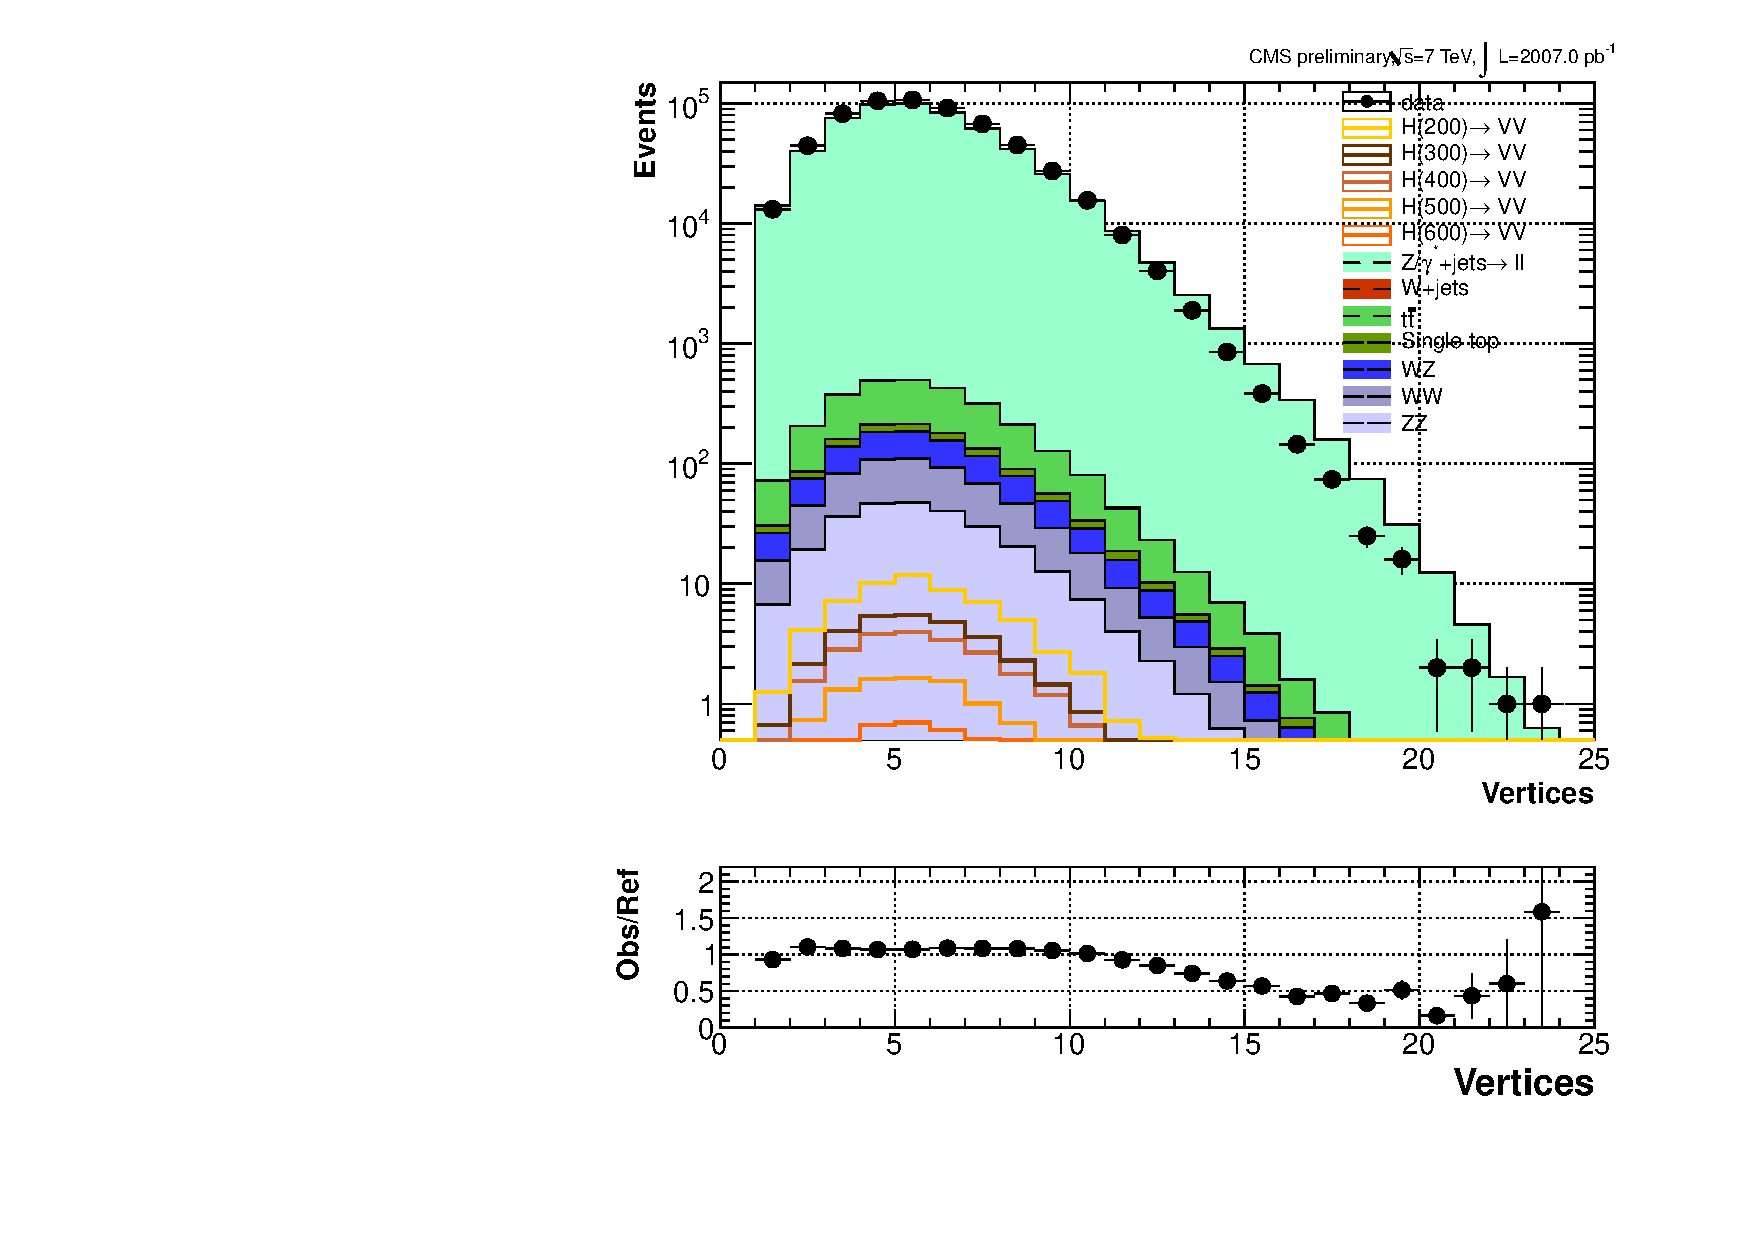
\includegraphics[width=0.4\textwidth]{img/mumu_ngoodvertex}
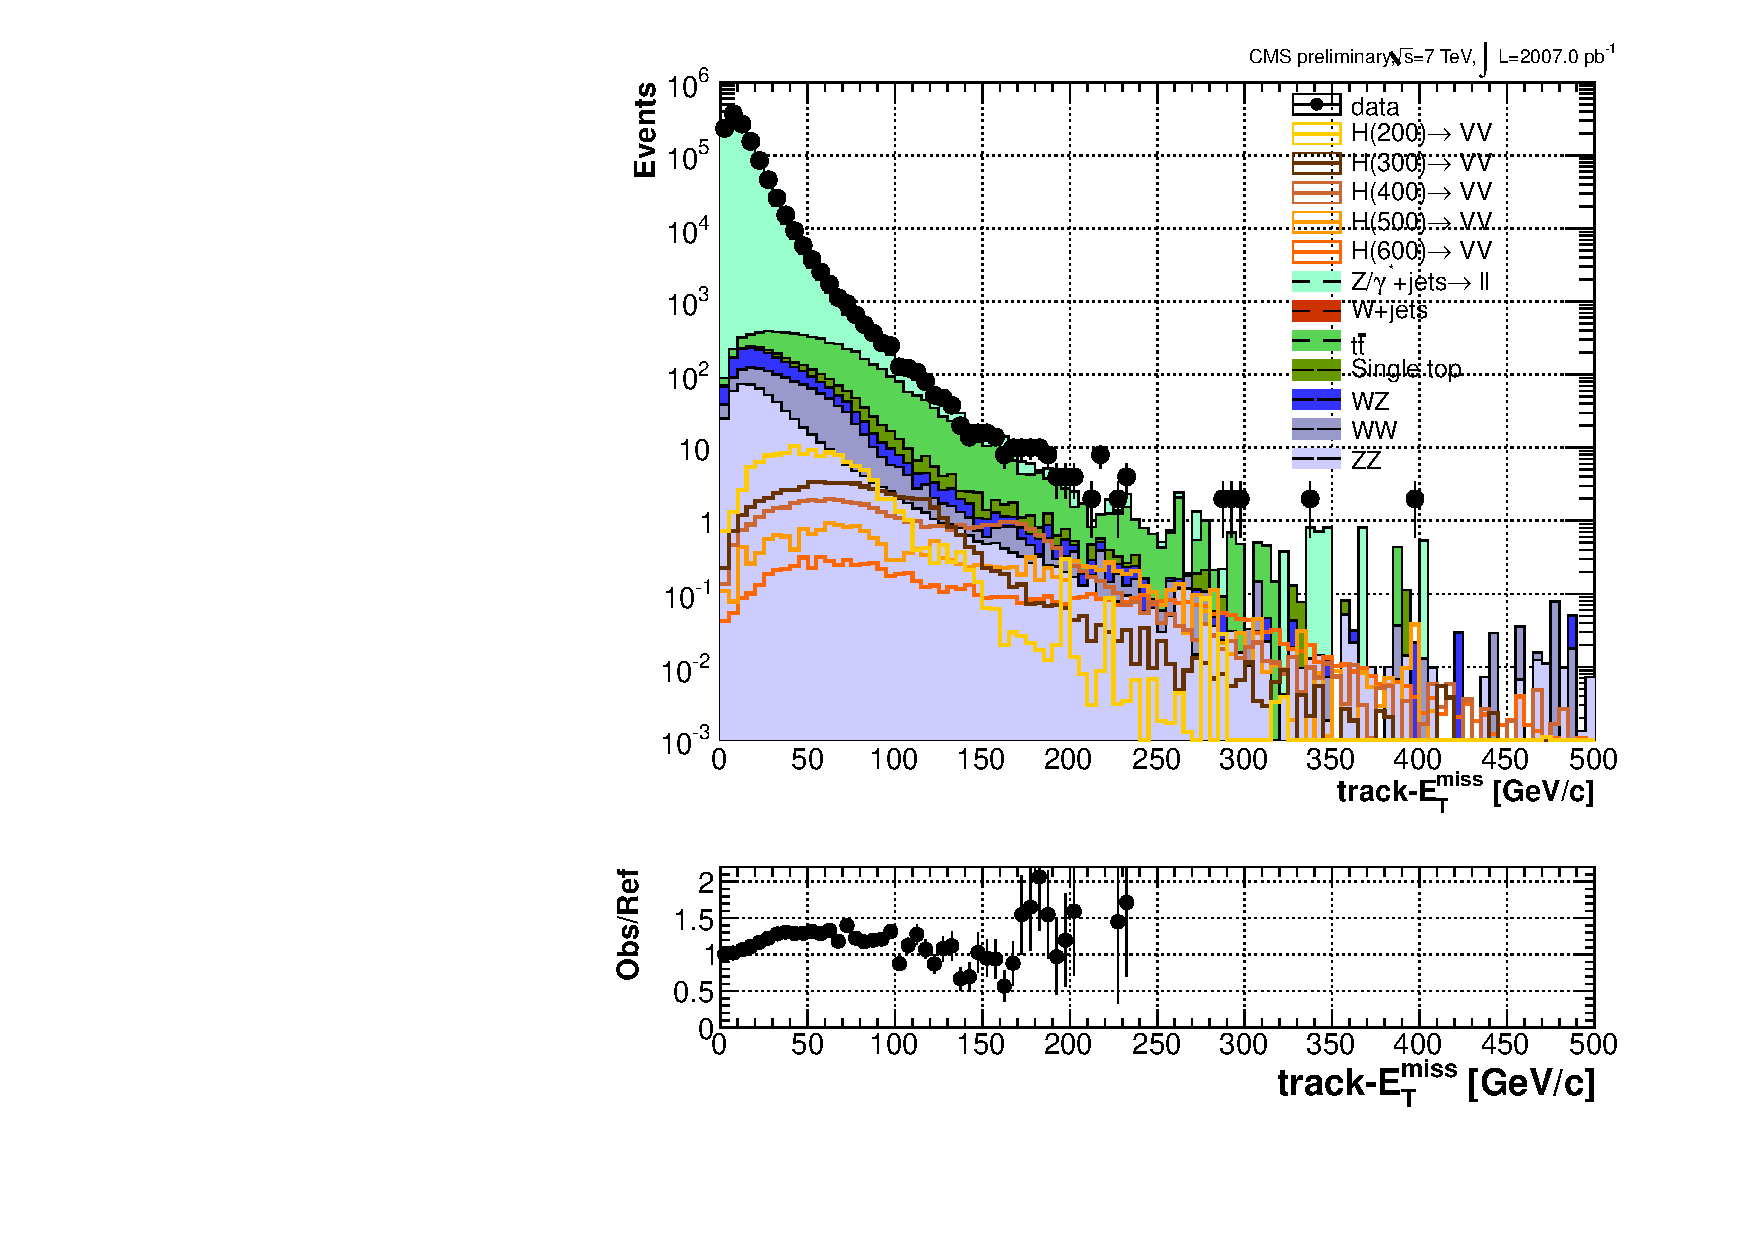
\includegraphics[width=0.4\textwidth]{img/mumu_trkmet}
\caption{Distribution of the vertex multiplicity ({\em left}) and the transverse momentum resulting from the sum of all charged particle-flow candidates associated to the primary vertex of the event ({\em right}).
The bottom plots show the ratio between the total MC prediction and the observed data.}
\label{fig:vertexcontrol}
\end{center}
\end{figure}




%%% LEPTONS
\item[Leptons] leptons (electrons or muons) are required to be reconstructed with at least $p_T>$5~GeV/c and $|\eta|<$2.5 (2.4) for electrons (muons). 

Electrons reconstructed in the ECAL barrel to endcap transition are not considered for this study in order to reduce the contamination from fakes and to 
minimize the impact of mismeasurement of the lepton energies which translates to a mismeasurement of the missing transverse energy of the event.
The impact parameter of the electron track is required to be consistent with prompt production from the beam spot within $|d_0|<$0.04~cm.
Non-prompt electrons, from photon conversions in the tracker material, are vetoed by geometric requirements
applied on partner tracks (dist$<$0.02~cm and $\Delta\cot\theta<$0.02) and by requiring a maximum of 1 lost tracker hit. 
For each electron it is also required that no tracker or global muon with at least 10 tracker hits is found within a $\Delta R<$0.1 of the reconstructed electron.
Electron identification relies on a simple cut based identification algorithm 
which depends on the supercluster shape, its alignment with the track which is associated to electron and H/E.
The electron-id cuts are tuned specifically for each ECAL region (barrel and endcap) in order to yield 
an expected efficiency for the reconstruction of electrons from $W\rightarrowe\nu$ decays.
Details on the VBTF specific requirements can be found in~\cite{CMS-TWIKI-VBTF11}.
For this study we require at pre-selection that the VBTF-95 working point is verified. 
For electron candidates to be considered as a leg of the dilepton candidate the verification of the VBTF-85 working point is further required
as well as having $p_T>$20~GeV/c. 
The choice on these electron-ids is trigger oriented, as the trigger identification requirements consist in looser versions of the VBTF requirements.

Muon identification is mainly based on the $\chi^2$ fit of the global track and on the number of hits in the tracker and muon stations.
Loose muons are required to verify the TrackerMuonArbitrated criteria, i.e. to be tracker muons, 
and to be consistent with prompt production from the beam spot within $|d_0|<$0.02~cm.
Basic tracker quality requirements are also imposed, namely that : $\chi^2/ndof<$10 and at least 11 tracker hits are used for the inner track fit.
In order to be considered as a leg of the dilepton candidate the muons are furthermore required 
to have 1 hit in the muon chambers and to verify the TMLastStationAngTight arbitration and have $p_T>$20~GeV.

The leptons from signal are expected to be well isolated in the event.
The isolation can be quantified relatively to the transverse momentum of the lepton by
sum of the momenta of the particles reconstructed in a cone of $\Delta R<0.3$ built around the lepton candidate.
The following measurement of the relative isolation is used, $I_{rel}$:

\begin{equation}
I_{rel}=\frac{I_{photons}+I_{neutral~hadrons}+I_{charged~hadrons}}{p_T}
\label{eq:reliso}
\end{equation}

where each $I$ represents the sum of the transverse momenta of the photons, neutral hadrons and charged hadrons reconstructed inside the isolation cone.
Loose electrons and muons are required to have $I_{rel}<$0.5. 
Electrons or muons are considered as legs of the dilepton candidate if they have $I_{rel}<0.1$.
In App.~\cite{sec:app:leptonisolation} the lepton isolation is discussed in further detail.

%%% DILEPTON
\item[Dilepton] for each event with at least 2 leptons selected in the previous conditions all dilepton pair candidates are examined.
The dilepton candidate is required to have an invariant mass compatible with a $Z$ boson decay, i.e. $|M-M_Z|<$15~GeV/c$^2$
and in case of ambiguity the pair with highest $\sum p_T$ is chosen.
No requirement is made on the charge of the leptons.
The reconstructed dilepton mass in the $Z$ boson acceptance window and the angle made by the two leptons in the transverse plane ($\Delta\phi$)
is shown in Fig~\ref{fig:dileptoncontrol}.

\begin{figure}[htp]
\begin{center}
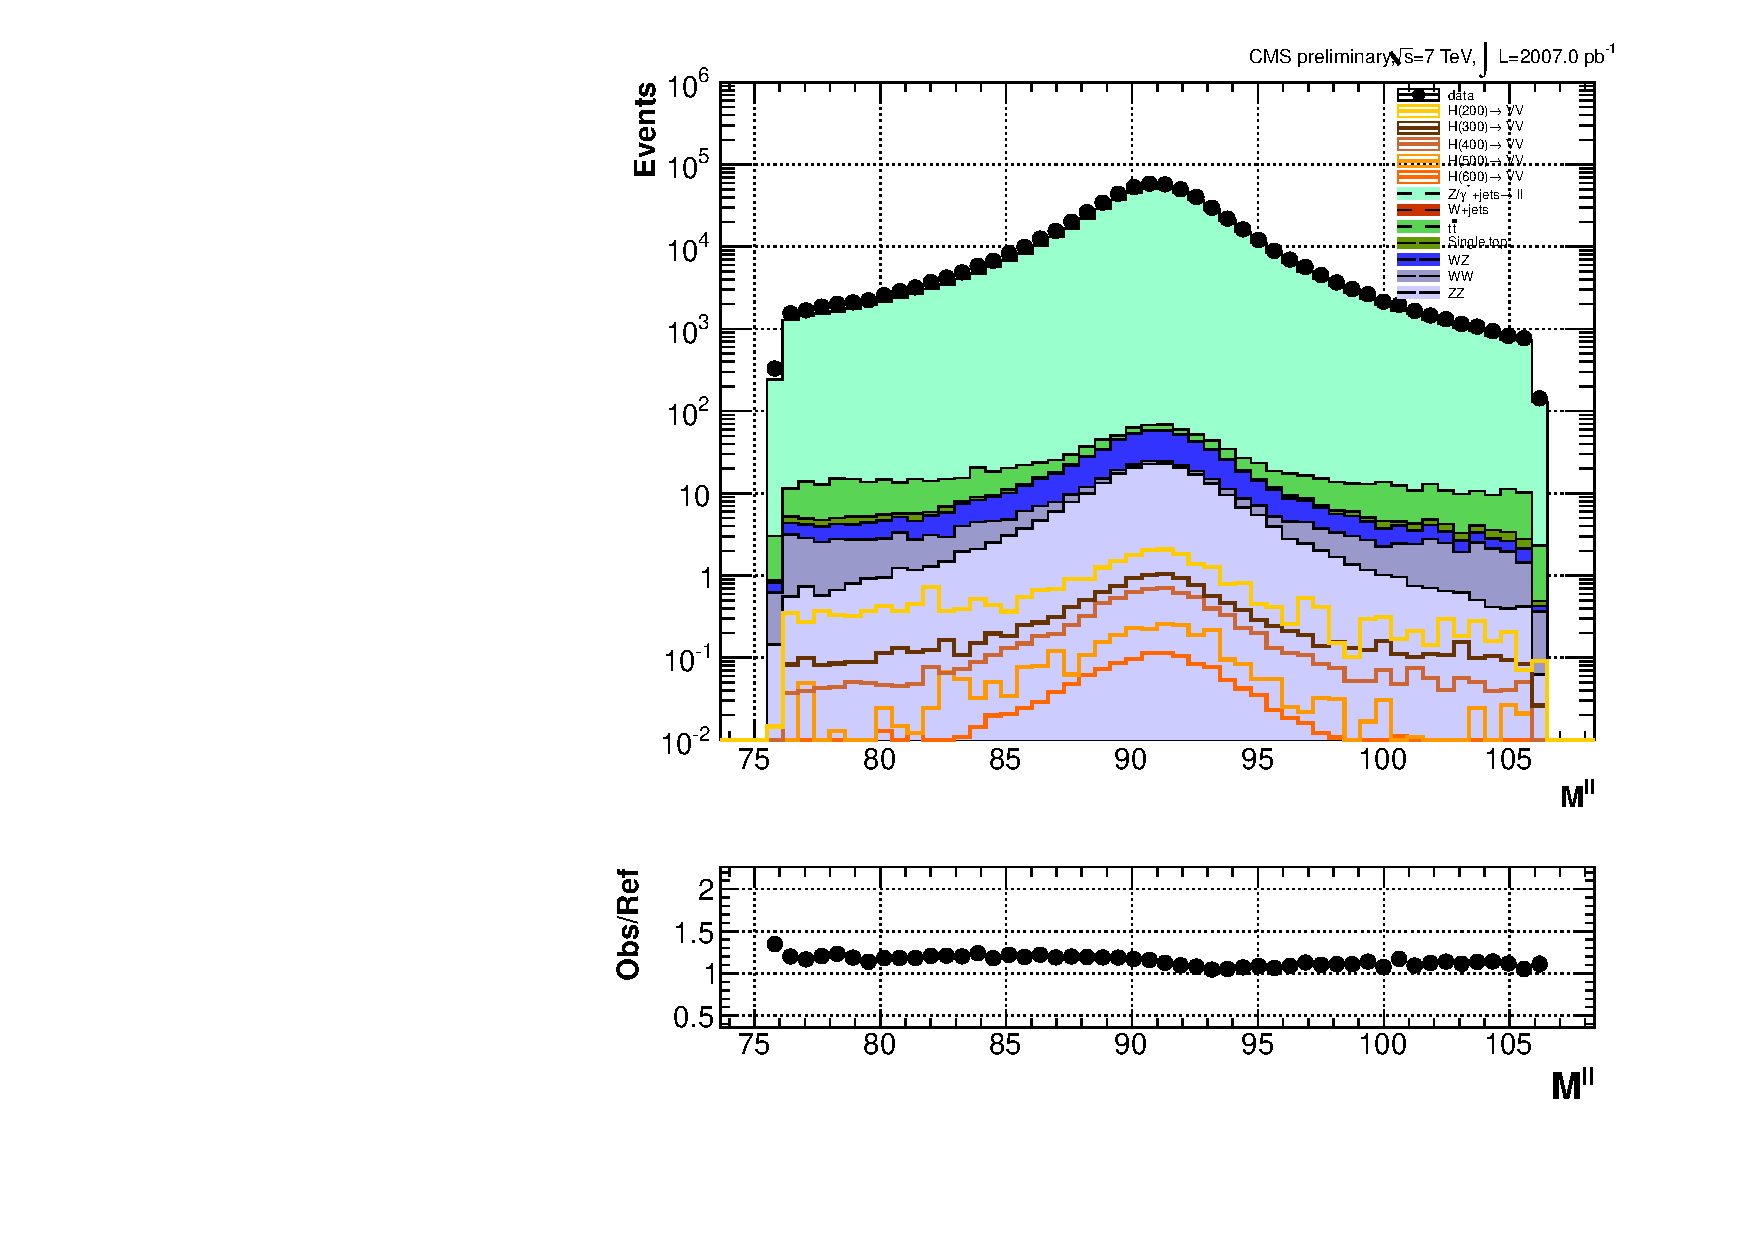
\includegraphics[width=0.4\textwidth]{img/mumu_recozmass}
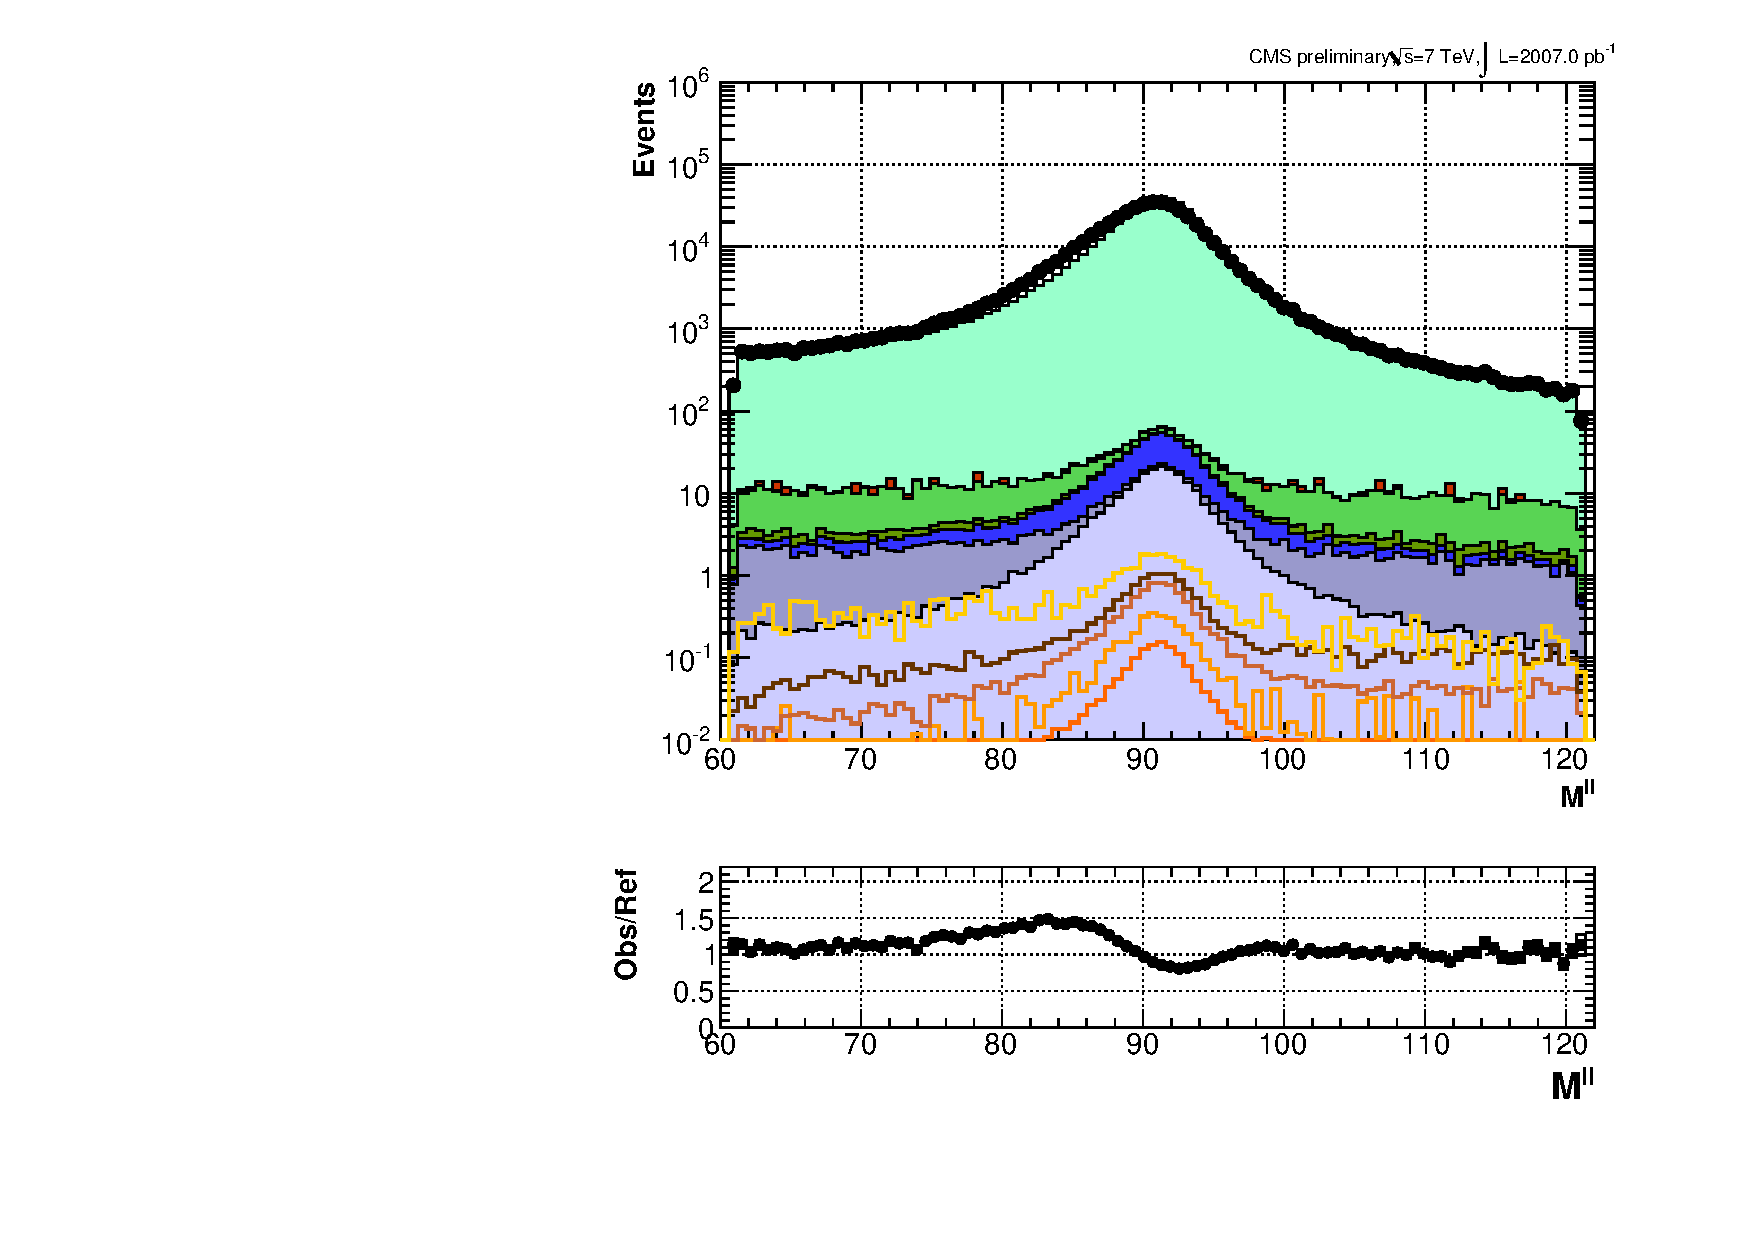
\includegraphics[width=0.4\textwidth]{img/ee_recozmass} \\
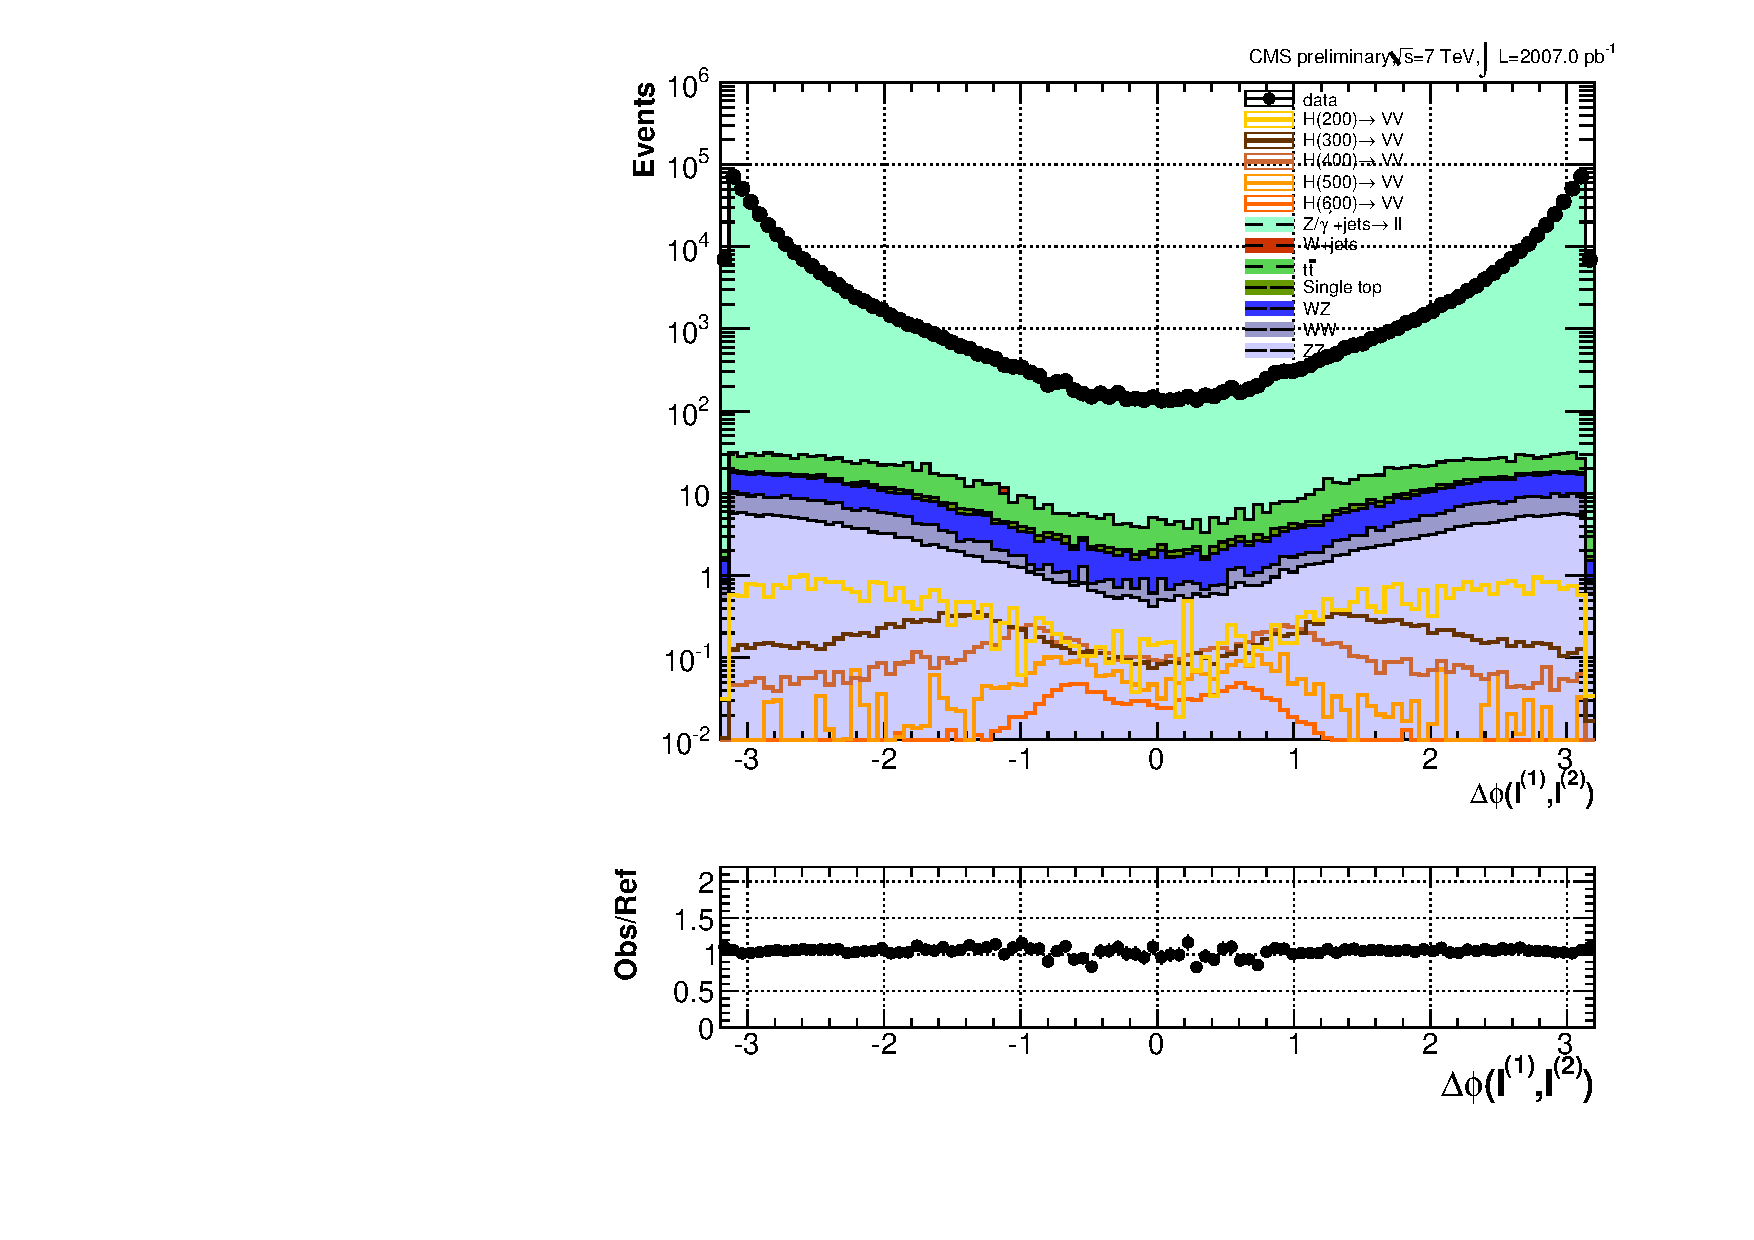
\includegraphics[width=0.4\textwidth]{img/mumu_recodphill}
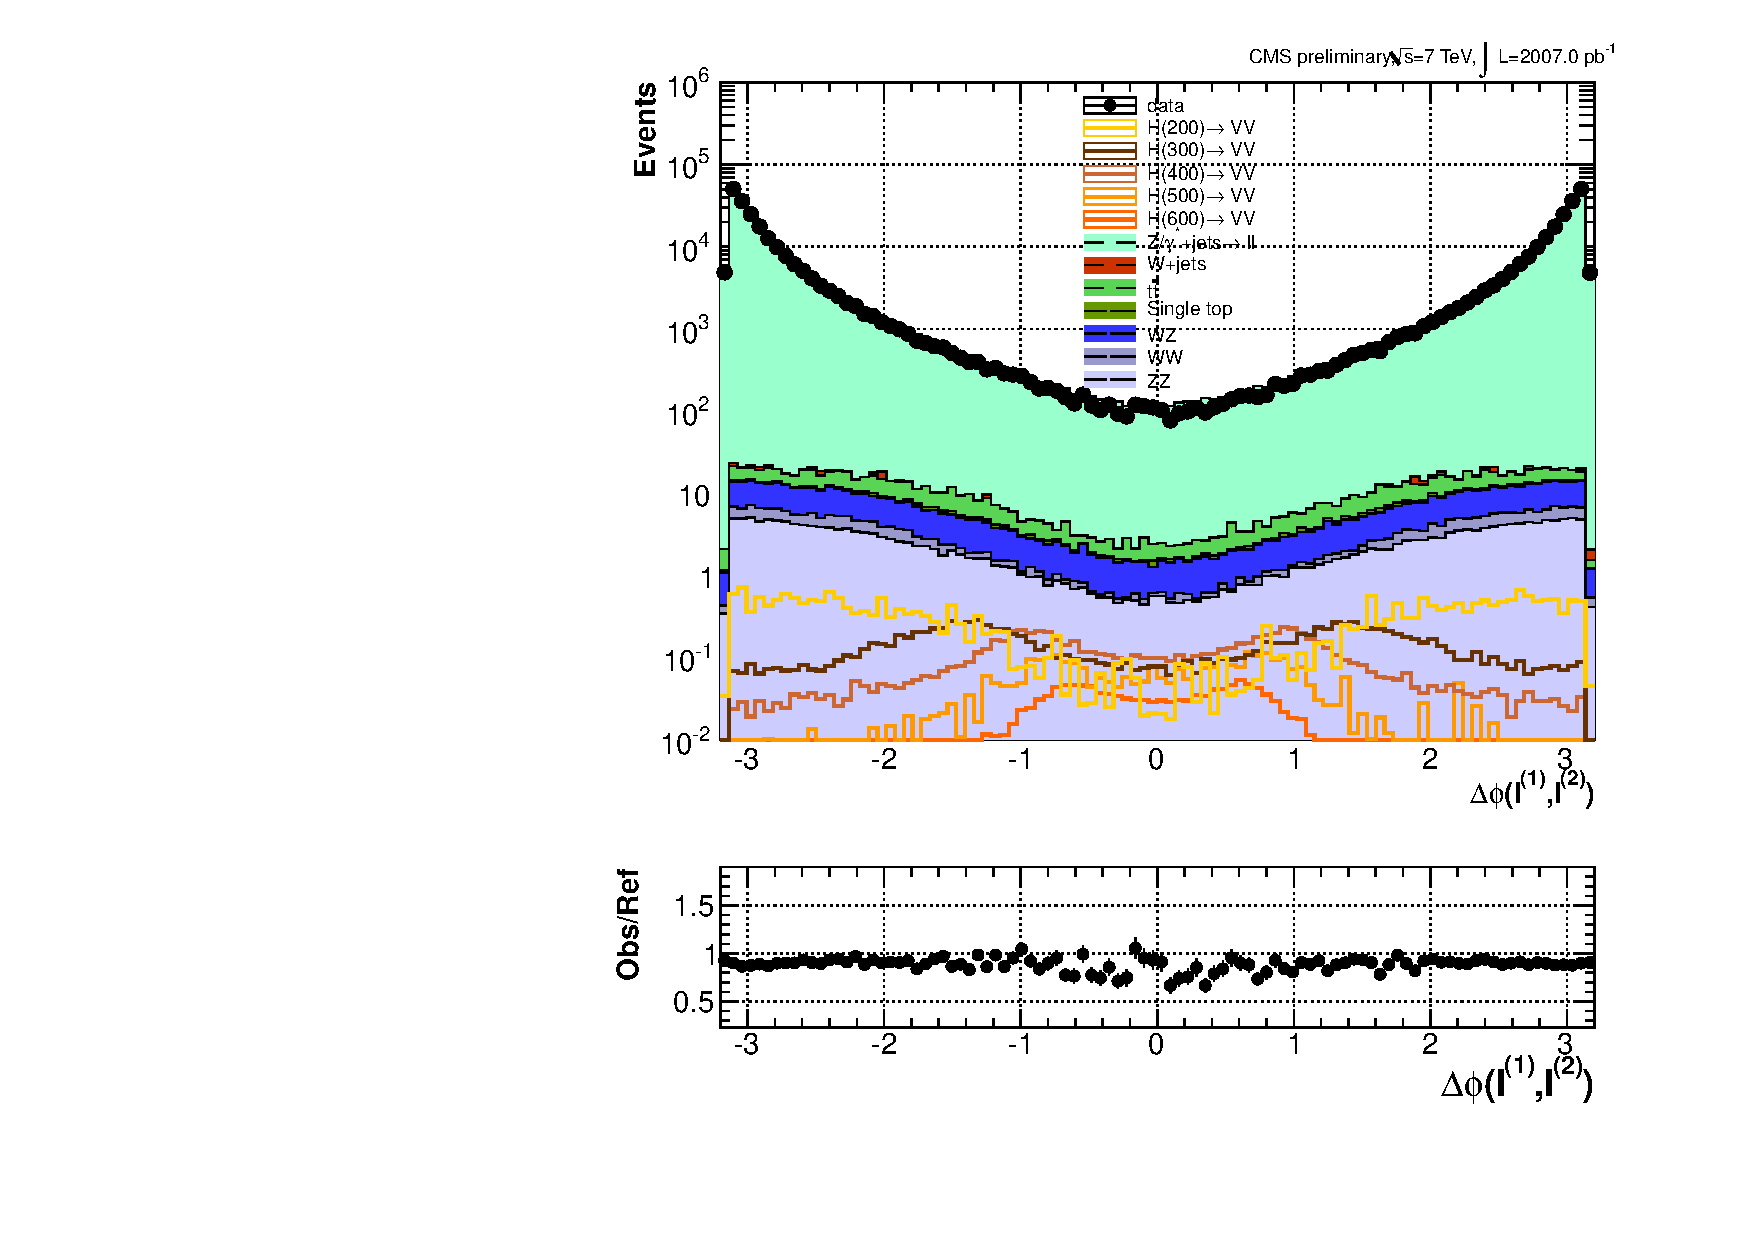
\includegraphics[width=0.4\textwidth]{img/ee_recodphill}
\caption{Lepton multiplicity distribution for di-muon ({\em left}) and di-electron ({\em right}) events with a mass compatible with the Z boson mass.}
\label{fig:dileptoncontrol}
\end{center}
\end{figure}

In order to reduce the contamination from multilepton events, produced from WZ and ZZ decays,
events are vetoed if containing another loosely selected electron or muon as described above.
The loose selection applied on the third lepton is expected to have a high efficiency for signal events($>$99.8\% for both channels).
The remainder of WZ and ZZ events are mostly due to fully hadronic decays of one of the vector bosons or to the decay of a Z boson to neutrinos.
A slight excess of events with more than 2 muons is observed in data as shown in Fig~\ref{fig:thirdleptonveto}
most probably related to a higher lepton fake rate than the one modelled by the MC.
Notice also that at this point no data-driven correction for the lepton efficiencies has been applied to correct further the MC.

\begin{figure}[htp]
\begin{center}
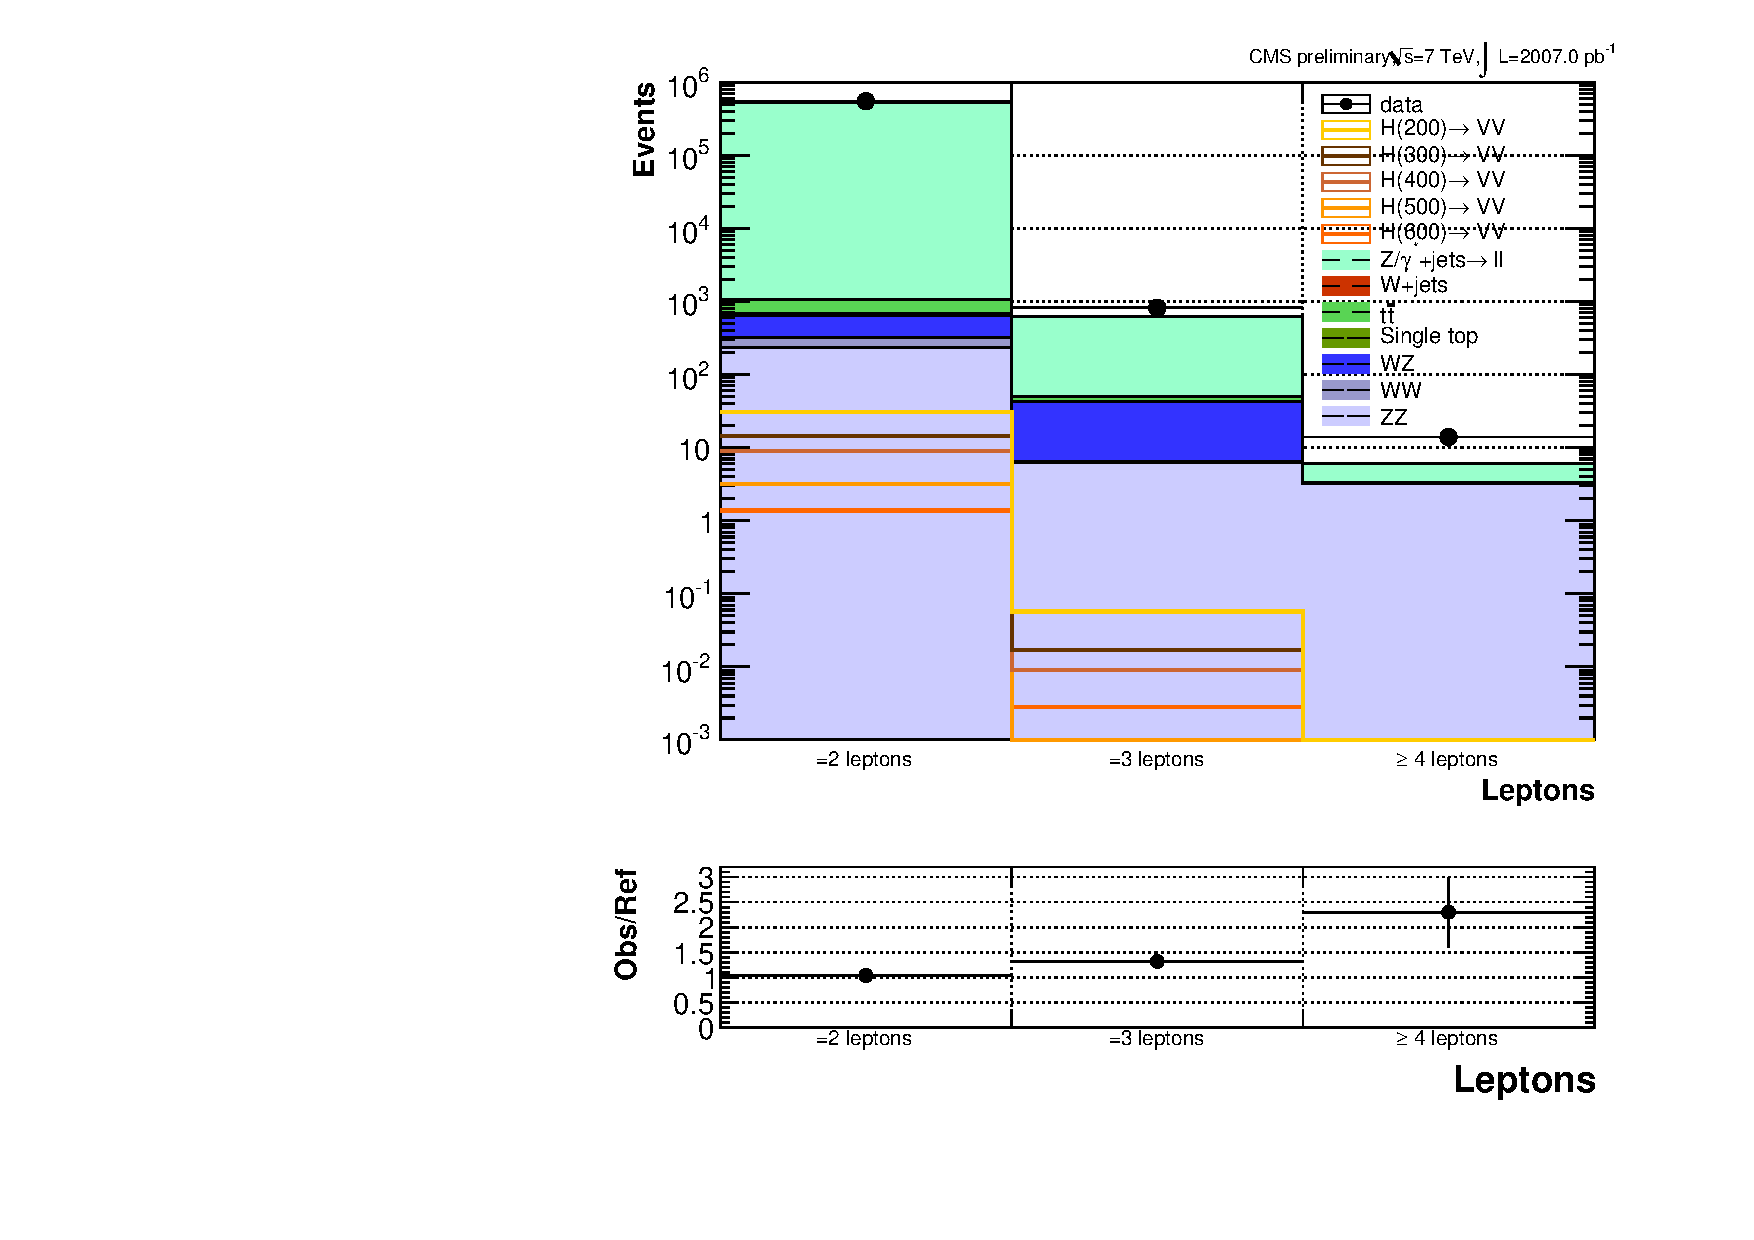
\includegraphics[width=0.4\textwidth]{img/mumu_nleptons}
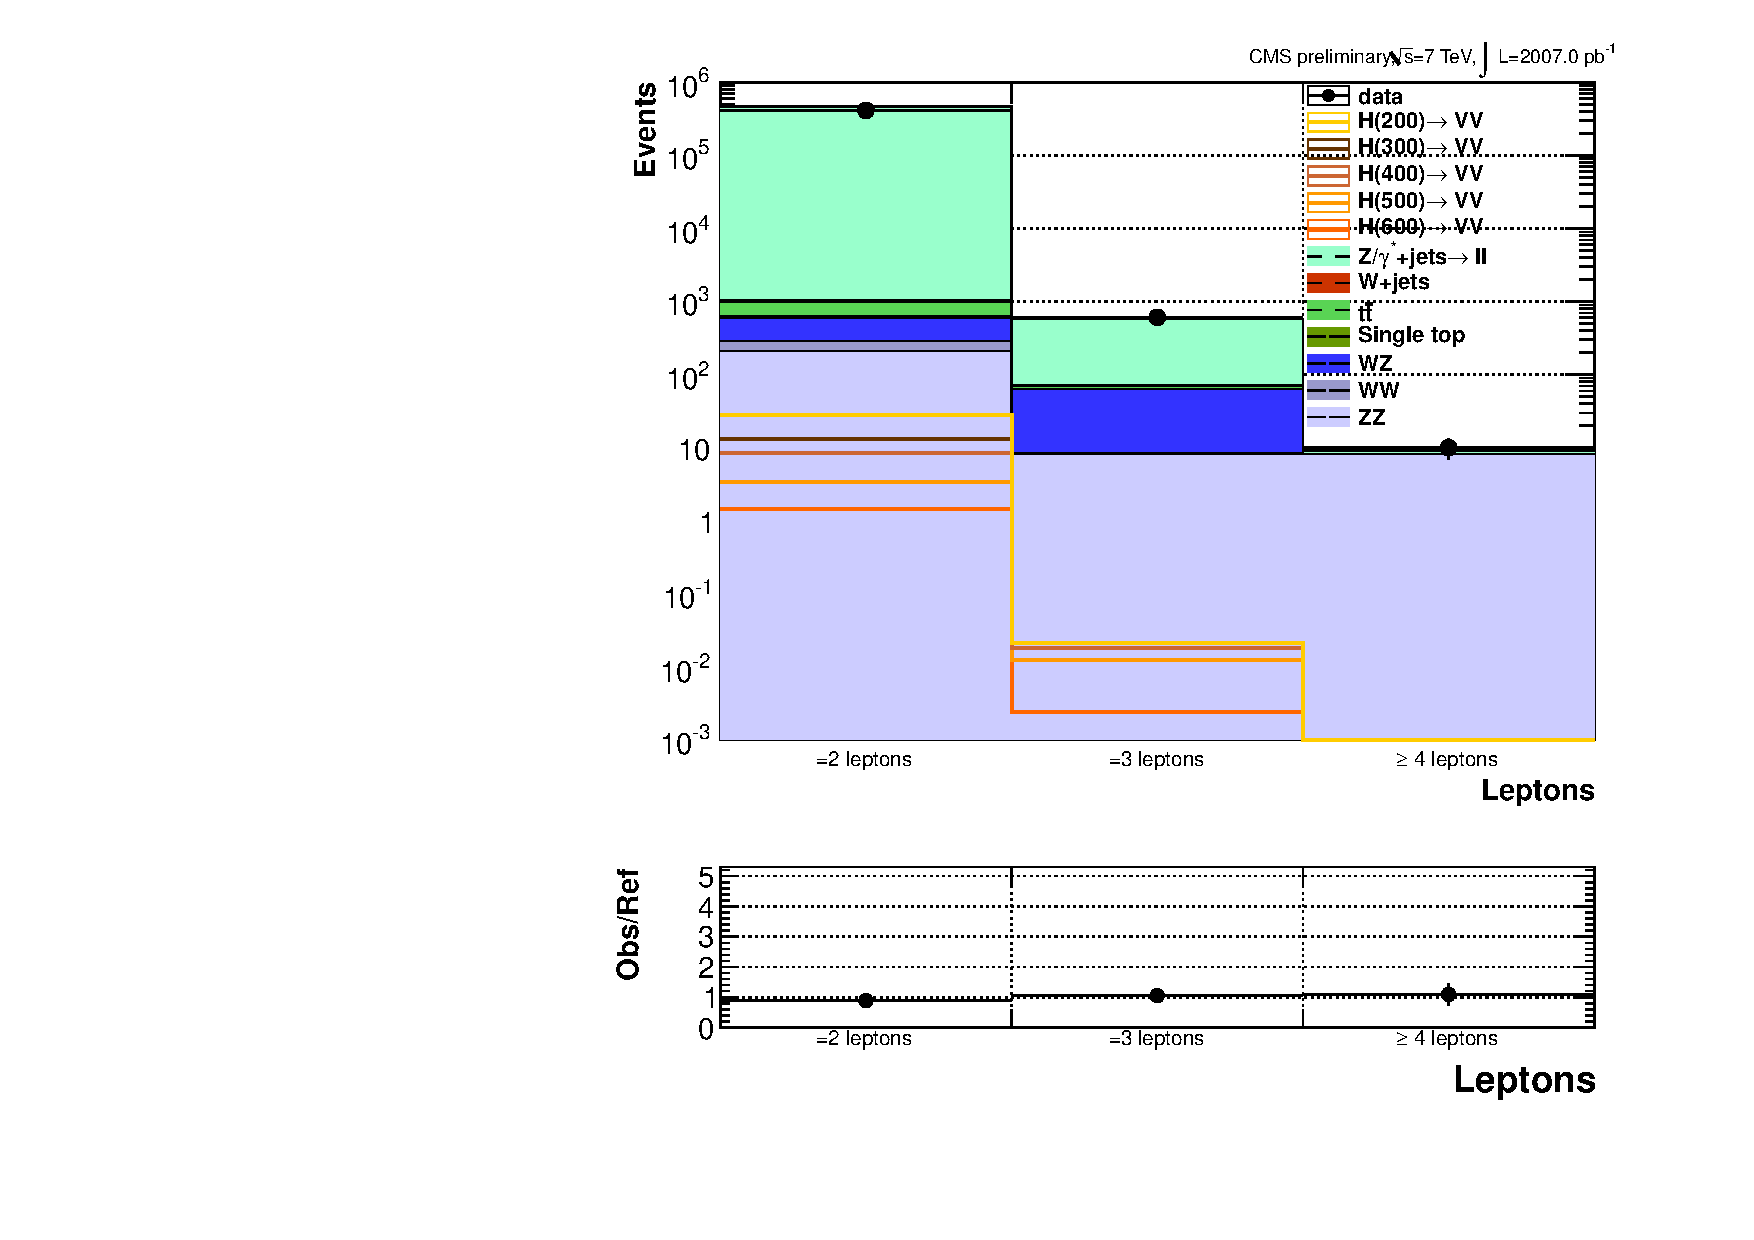
\includegraphics[width=0.4\textwidth]{img/ee_nleptons}
\caption{Lepton multiplicity distribution for di-muon ({\em left}) and di-electron ({\em right}) events with a mass compatible with the Z boson mass.}
\label{fig:thirdleptonveto}
\end{center}
\end{figure}



%%% JETS
\item[Jets] are reconstructed with the anti-$k_T$ algorithm with a cone of $R=0.5$ are selected with $p_T>$15~GeV/c and $|\eta|<5.0$.
The loose jet id used to select the jets is based on the electromagnetic fraction of the jets among other variables.
In order to reduce the contamination from processes which produce heavy flavor jets such as \ttbar, single top, vector boson + heavy quarks production,
b-tagging algorithms are used.
The jet-B probability (JBP) and the simple secondary vertex high efficiency (SSVHE) taggers are used for this purpose. 
Details of these algorithms and their performance can be found in~\cite{CMS-PAS-BTV-11-001}.
Events with a jet with $p_T>$30~GeV/c, tagged with the loose working point of the JBP algorithm or with the medium working point of the SSVHE algorithm, are rejected. 
This choice is made after optimizing the efficiency of the rejection of the top contribution.

%%% MET
\item[Missing transverse energy] particle flow based \MET is used. The \MET is built from the vectorial sum of the transverse momentum all particle flow reconstructed candidates.
The verification of the reconstruction of the missing transverse energy will be the subject of a detailed discussion in Sec.~\ref{sec:met}.

\end{description}

In the next section the event yields after pre-selection of the sample and control plots are presented for the main variables of interest.


%%
%% EVENT YIELDS
%%
\subsection{Event yields}
\label{subsec:eventyields}

The event yields after applying the pre-selection discussed in the previous section
are shown in Tables~\ref{tab:presamplecutflow}.

\begin{table}[htp]
\caption{Event yields for a total integrated luminosity of 1091~pb$^{-1}$. The uncertainties quoted are statistical only.}
\label{tab:presamplecutflow}
\begin{center}
\begin{tabular}{lccc} \hline\hline
Process                            & $|M-M_Z|<$15 & 3$^{rd}$-lepton veto & no b-tags\\ \hline
& & & \\\hline
\multicolumn{4}{c}{\bf $\mu\mu$ channel} \\\hline
ZZ                                 & $ 39.17 \pm0.28 $  & $ 39.17 \pm0.28 $  & $ 38.65 \pm0.28 $ \\
WW                                 & $ 67.4 \pm1.6 $  & $ 67.3 \pm1.6 $  & $ 66.6 \pm1.6 $  \\
WZ                                 & $ 73.3 \pm0.7 $  & $ 52.9 \pm0.6 $  & $ 51.5 \pm0.6 $  \\
Single top                         & $ 27.4 \pm0.7 $  & $ 27.1 \pm0.7 $  & $ 11.1 \pm0.4 $  \\
$t\bar{t}$                         & $ 303 \pm5 $  & $ 302 \pm5 $  & $ 66.5 \pm2.3 $  \\
W+jets                             & $ 0.32 \pm0.32 $  & $ 0.32 \pm0.32 $  & $ 0.32 \pm0.32 $ \\
$Z/\gamma^{*}+jets\rightarrow ll$  & $ ( 393.2 \pm0.5 ) \times10^{3} $  & $ ( 392.9 \pm0.5 ) \times10^{3} $  \\
Total expected                     & $ ( 393.7 \pm0.5 ) \times10^{3} $  & $ ( 393.3 \pm0.5 ) \times10^{3} $  & $( 388.3 \pm0.5 ) \times10^{3}$ \\ \hline
data                               & $ 328.5 \times10^{3} $  & $ 328.1 \times10^{3} $  & $  324.1 \times10^{3}$ \\ \hline
& & & \\\hline
\multicolumn{4}{c}{\bf $ee$ channel} \\\hline
ZZ                                 & $ 31.35 \pm0.25 $  & $ 31.32 \pm0.25 $  & $ 30.95 \pm0.25 $  \\
WW                                 & $ 55.4 \pm1.4 $  & $ 55.3 \pm1.4 $  & $ 54.6 \pm1.4 $  \\
WZ                                 & $ 80.6 \pm0.7 $  & $ 44.4 \pm0.5 $  & $ 43.4 \pm0.5 $  \\
Single top                         & $ 24.1 \pm0.6 $  & $ 23.8 \pm0.6 $  & $ 9.9 \pm0.4 $  \\
$t\bar{t}$                         & $ 259 \pm5 $  & $ 257 \pm5 $  & $ 57.8 \pm2.2 $ \\
W+jets                             &  $ 57 \pm8 $  & $ 57 \pm8 $  & $ 55 \pm8 $  \\
$Z/\gamma^{*}+jets\rightarrow ll$  & $ ( 313.1 \pm0.4 ) \times10^{3} $  & $ ( 312.8 \pm0.4 ) \times10^{3} $  & $ ( 308.8 \pm0.4 ) \times10^{3} $ \\
Total expected                     & $ ( 313.6 \pm0.4 ) \times10^{3} $  & $ ( 313.2 \pm0.4 ) \times10^{3} $  & $ ( 309.0 \pm0.4 ) \times10^{3} $ \\\hline
data                               & $ 265.6 \times10^{3} $  & $ 265.2 \times10^{3} $  & $  261.9 \times10^{3} $  \\\hline\hline
\end{tabular}
\end{center}
\end{table}

%%
%%
%%
\section{Verification of the reconstructed missing transverse energy}
\label{sec:met}

%%%
%%% Pileup
%%%
\subsection{Strategies adopted to minimize the effect of pileup}
\label{subsec:pueffects}

\begin{table}[htp]
\caption{}
\label{tab:mettypes}
\begin{center}
\hspace*{-2cm}
\begin{tabular}{llllllll} \hline\hline
\multicolumn{2}{c}{\MET components}                  & PF     & PF no pileup  & track PF              & charged PF & clust. neut. & jet vetoed neut.  \\\hline
\multirow{2}{*}{charged}            & all                      & yes    & -             & -                     & -          & -            & -                    \\
                                    & from PV ($\Delta Z<$cm)  & -      & yes           & yes                   & yes        & yes          & yes                  \\\hline
\multirow{2}{*}{neutrals}           & all                      & yes    & yes           & $p_T>4 \wedge \eta<3$ & no         & no           & yes                  \\
                                    & associated to PV jets    & -      & -             & -                     & -          & yes          & -                    \\
                                    & associated to other jets & -      & -             & -                     & -          & -            & no                   \\\hline\hline
\end{tabular}
\end{center}
\end{table}


%%%
%%% REDUCED MET
%%%
\subsection{Description of the reduced \MET method}
\label{subsec:redmet}

We adopt the definition of reduced missing transverse energy (\RMET) for our analysis.
The definiton is an upgrade of the original concept developed by the D0 collaboration~\cite{Abazov:2008yf}.
The reconstructed \MET is decomposed using either the dilepton direction (in case the two leptons are collimated,
i.e. $\Delta\phi^{ll}<\pi/2$) or the dilepton bisector (in case the two leptons are reconstructed with an open angle,
i.e.   $\Delta\phi^{ll}>\pi/2$).
The bisector of the dilepton is defined transversely to the axis which maximizes the dilepton transverse momentum, 
i.e. the thrust axis($\vec{t}$):

\begin{equation}
\vec{t} =\frac{1}{|\vec{l}_1-\vec{l}_2|}(\vec{l}_1 - \vec{l}_{2})
\label{eq:thrust} 
\end{equation}

where $l_{i}$ is the momentum of the $i$-th lepton. The bisector ($\vec{b}$) is defined in such a way that:

\begin{equation}
\vec{b}\cdot\vec{t}=0 ~~~\wedge~~~ \vec{b}\cdot\vec{l}_1>0
\label{eq:bisector} 
\end{equation}

The thrust and bisector are used to define the projections of the recoil from the jets
(clustered recoil) and the \MET (unclustered recoil) as:

\begin{equation}
R^{\text{clustered}}_{i}=(\sum_{jets} \vec{p}_T) \cdot \hat{i} ~~~~~~~ R^{\text{unclustered}}_{i}=pfMET \cdot \hat{i}
\label{eq:dilrecoilcomponents}
\end{equation}

where $i=t,b$ as defined in Eqs.~\ref{eq:thrust} and ~\ref{eq:bisector}.  
\RMET is defined from the minimum imbalance found using either the clustered or the unclustered recoil of the system.
Each component of \RMET is computed and minimized individually:

\begin{equation}
{\rm red}\cancel{E}_{T_i}^{k} =\vec{p}_{T}^{ll}\cdot \vec{i} + \alpha R^{\text{k}}_{i}
\label{eq:rmet}
\end{equation}

where k=clustered/unclustered. The absolute \RMET measurement is taken from the quadratic sum of the two components.
The procedure just described assumes a conservative scenario for jet energy and unclustered \MET reconstruction and resolution.
It is also expected to be effective against pileup events as jets are seeded using particle flow candidates associated to the
primary vertex selected for each event. Table~\ref{tab:metwp} summarizes the performance of different \MET approaches
regarding the rejection of the Drell-Yan background and the selection of a standard model Higgs with a mass of 200 GeV/$c^{2}$.

\begin{table}[htp]
\caption{Working points for different Drell-Yan rejection powers for standard \MET, projected-\MET and \RMET.}
\label{tab:metwp}
\begin{center}
\begin{tabular}{llll} \hline\hline
\MET                  & PF      & projected  & reduced  \\\hline
                      &        &         & \\
\multicolumn{4}{c}{Medium working point ($10^{-3}$ rejection factor)} \\\hline
Cut value             & 48.4    & 44.1       & 38.9  \\
H(200)                & 49.6\%  & 40.7\%     & 53.2\%  \\\hline
                      &         &             & \\
\multicolumn{4}{c}{Tight working point ($10^{-4}$ rejection factor)} \\\hline
Cut value             & 66.5    & 63.9       & 56.7 \\
H(200)                & 27.5\%  & 20.9\%     & 30.0\% \\\hline\hline
\end{tabular}
\end{center}
\end{table}

%%
%%
%%
\subsection{Data-driven estimation of the instrumental background}
\label{subsec:instrumentalbackground}

Photon candidates are selected from dedicated photon triggered samples.
The samples are summarized in Table~\ref{tab:instrbckgdatasamples}.

\begin{table}[htp]
\begin{center}
\caption{MC and data samples analyzed for the estimation of the instrumental background.
For data the total integrated luminosity and the run range analyzed are shown.
For MC the the cross section and the corresponding integrated luminosity of the analyzed sample are shown.
Z2 is used as a shortname for TuneZ2\_7TeV\_pythia6 and S* for Summer11-PU\_S*\_START42\_V11.
}          
\label{tab:instrbckgdatasamples}
\begin{tabular}{lcl} \hline\hline
\multicolumn{3}{c}{\bf Data} \\
Dataset                               & $L$~(pb$^{-1}$)               & Run range                          \\\hline
/Photon/Run2011A-May10ReReco-v1/AOD   &                               & {\small 160404-163869}             \\
/Photon/Run2011A-PromptReco-v4/AOD    &                               & {\small $>$163869}                 \\
{\bf Total}                           & {\bf }                        &                                    \\\hline
                                      &                               &                                    \\\hline
\multicolumn{3}{c}{\bf MC} \\
Dataset                               & $\sigma$~(pb)                 & $L$~(pb$^{-1}$)                   \\\hline
/G\_Pt-15to30\_Z2/S3-v2/AODSIM        & 1.72$\times$10$^5$            &                                   \\
/G\_Pt-30to50\_Z2/S3-v2/AODSIM        & 1.67$\times$10$^4$            &                                   \\
/G\_Pt-50to80\_Z2/S3-v2/AODSIM        & 2.72$\times$10$^3$            &                                   \\
/G\_Pt-80to120\_Z2/S4-v2/AODSIM       & 4.47$\times$10$^2$            &                                   \\
/G\_Pt-120to170\_Z2/S3-v2/AODSIM      & 84.2                          &                                   \\
/G\_Pt-170to300\_Z2/S4-v2/AODSIM      & 22.6                          &                                   \\
/G\_Pt-300to470\_Z2/S3-v2/AODSIM      & 1.49                          &                                   \\
/G\_Pt-470to800\_Z2/S3-v2/AODSIM      & 0.132                         &                                   \\
/G\_Pt-800to1400\_Z2/S3-v2/AODSIM     & 3.48$\times$10$^{-3}$         &                                   \\
/G\_Pt-1400to1800\_Z2/S3-v2/AODSIM    & 1.26$\times$10$^{-5}$         &                                   \\\hline\hline
\end{tabular}
\end{center}
\end{table}

For each triggered event the highest $p_T$ photon trigger candidate is chosen.
The offline reconstructed photon is required to have a $E_T$ 
greater than that of the trigger threshold it fired.
Further identification and isolation requirements are made as summarized in Table~\ref{tab:photonsel}
and are based on~\cite{Khachatryan:2010fm}.

\begin{table}[htp]
\begin{center}
\caption{Photon selection requirements according to the region of reconstruction in the electromagnetic calorimeter.}
\label{tab:photonsel}
\begin{tabular}{lcc} \hline\hline
Variable                              & ECAL barrel                        & ECAL endcap                   \\\hline
$E_T$                                 & \multicolumn{2}{c}{trigger dependent}                              \\
$|\eta|$                              & $<$1.4442                          & 1.566$<|\eta|<$2.5            \\ 
$\sigma_{i\eta i\eta}$                & 0$<\sigma<$0.013                   & 0$<\sigma<$0.03               \\ 
$\sigma_{i\phi i\phi}$                & $>$0                               & -                             \\ 
seed rec. hit flag                    & $\neq$ kOutOfTime                  & -                             \\ 
$h/e$                                 & $<$0.05                            & $<$0.5                        \\ 
Tracker isolation                     & \multicolumn{2}{c}{$<$2.0 + 0.001$E_T$}                            \\ 
ECAL isolation                        & \multicolumn{2}{c}{$<$4.2 + 0.003$E_T$}                            \\ 
HCAL isolation                        & \multicolumn{2}{c}{$<$2.2 + 0.001$E_T$}                            \\\hline 
\end{tabular}
\end{center}
\end{table}

%
%
%
\section{Search for the standard model Higgs in the 2l2$\nu$ final state}
\label{sec:higgssearch}


%%
%% Higgs event selection
%%
\subsection{Higgs event selection}
\label{subsec:higgsselection}


%%
%% Discriminator analysis
%%
\subsection{Discriminator based analysis of the selected events}
\label{subsec:discanalysis}

%%
%% Background determination
%%
\subsection{Background determination}
\label{subsec:backgrounddet}

%%
%%
%%
\subsection{Efficiency of the selection}
\label{subsec:selefficiency}

%%
%%
%%
\subsection{Systematic uncertainties}
\label{subsec:systunc}


%
%
%
\section{Exclusion limits}
\label{sec:excllimits}


%
% CONCLUSIONS
%
\section{Conclusions}
\label{sec:conclusions}

%% **DO NOT REMOVE BIBLIOGRAPHY**
\bibliography{auto_generated}   % will be created by the tdr script.

\clearpage
%
% APPENDIX
%
\appendix
\section{Appendix: Lepton isolation}
\label{sec:app:leptonisolation}

In this section we focus on two specific aspects affecting the determination of lepton isolation efficiency:
the contamination from pileup and the differences between leptons in the $Z\rightarrow ll$ sample and in the Higgs sample.

The presence of pileup is expected to contribute to the degradation of the isolation, especially 
through the neutral particles which cannot be associated to the vertex.
The deviation introduced in the isolation by the average energy density deposition in the detector from pileup
can be estimated using the $\rho$-parameter computed using the fast jet algorithm~\cite{Cacciari:2007fd}.
As the average values for $\rho$, $I_{photons}$ and $I_{neutral~hadrons}$ are expected to increase differently as a function of the number of pileup events
a linear parameterization can be derived for each case and used to correct the isolation in average.
The results of these parameterizations are shown for in Fig~\ref{fig:isolprofile} for a simulated sample of $Z\rightarrow \mu\mu$.
The width of the distributions of the previous variables is also affected by the pileup and in the case of the $\rho$ a non-linear behavior is observed.
In this study we choose therefore not to perform any correction for the isolation based on the pileup contamination as estimated from 
the $\rho$ parameter due to the fact that events with large fluctuations of $\rho$ can lead to overcorrections of the lepton isolation leading to an increase
of the contamination from non-isolated lepton candidates.
The slope of the isolation profile is used to assign a systematic uncertainty on the isolation efficiency of 0.8\%
for both electrons and muons.

\begin{figure}[htp]
\begin{center}
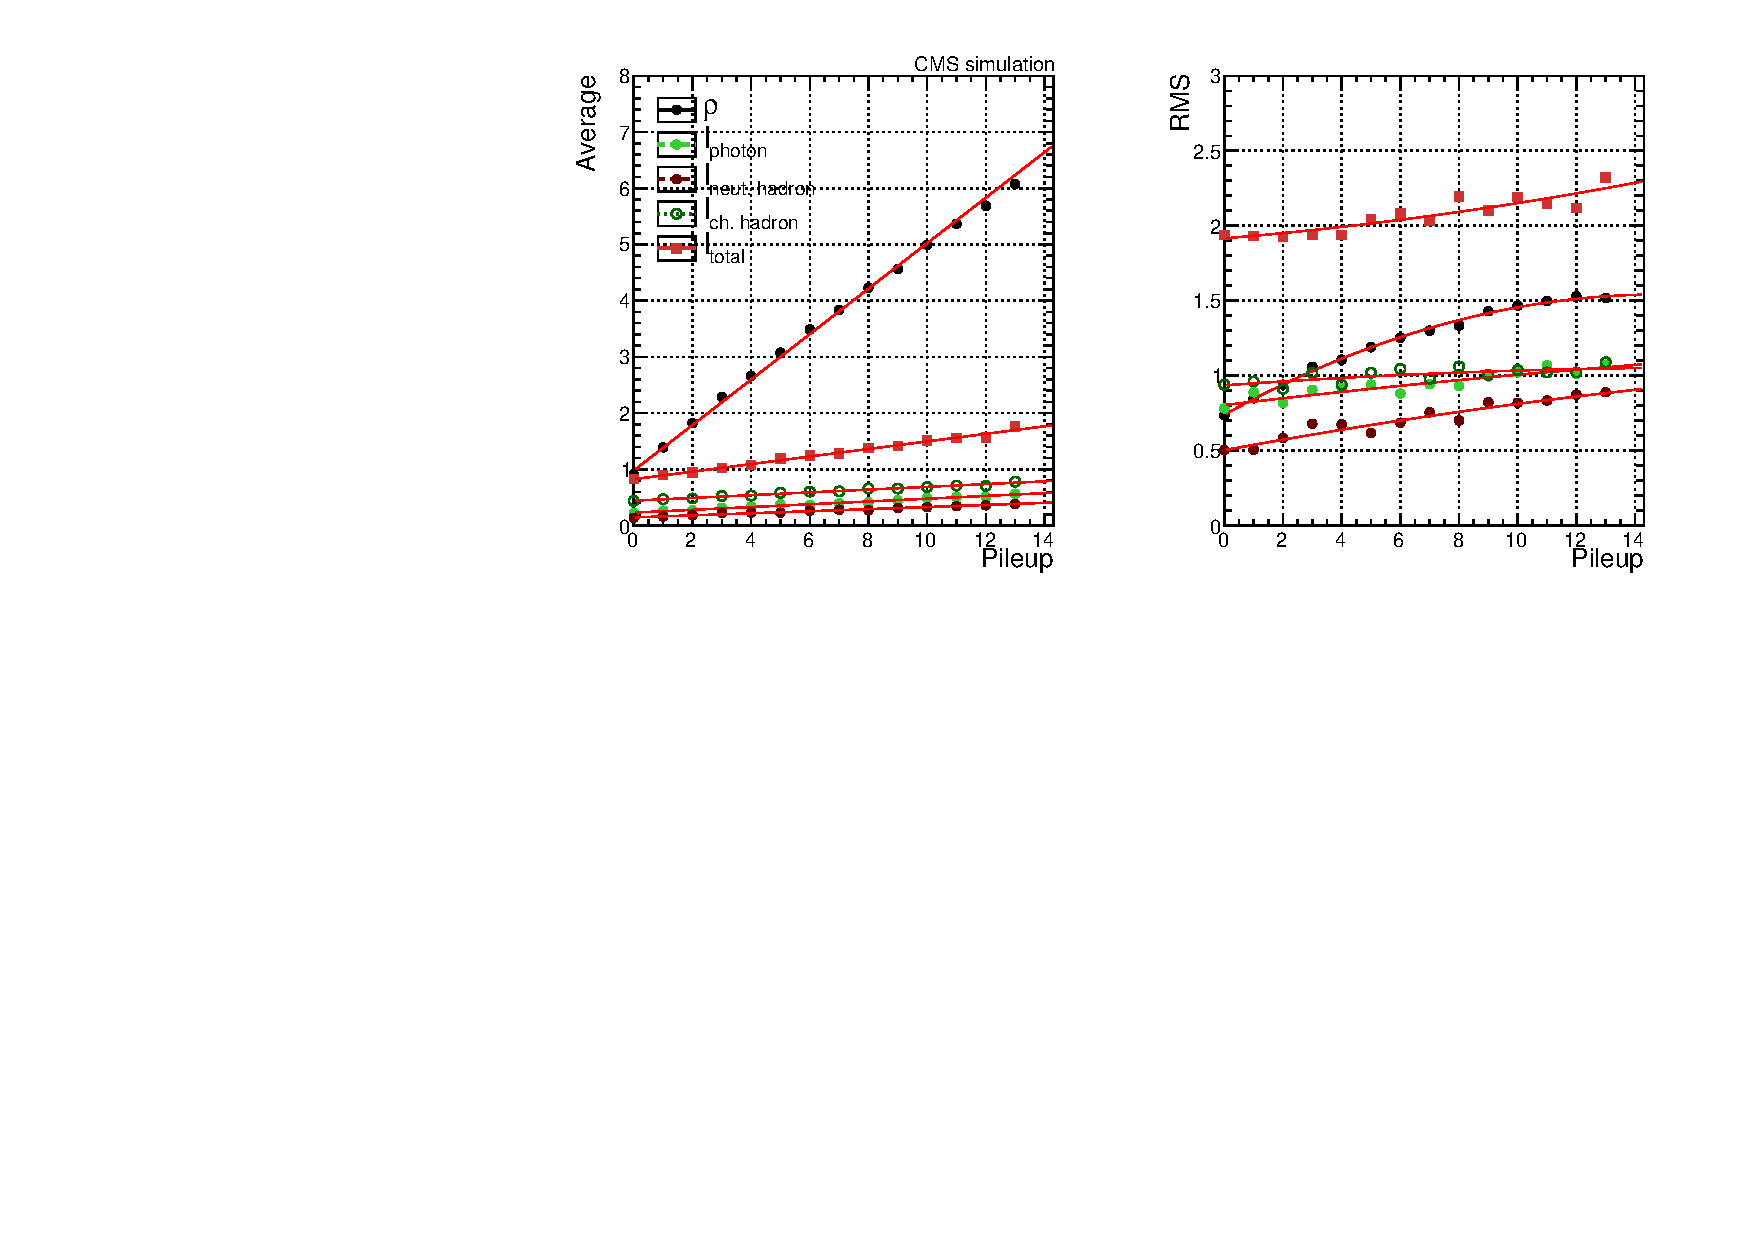
\includegraphics[width=0.9\textwidth]{img/muonIsolationProfile}
\caption{
Isolation and $\rho$ profiles in simulated $H\rightarrow VV\rightarrow 2\mu 2\nu_{\mu}$ events.
The average (RMS) of the distributions is shown as function of the number of generated pileup events on the {\em left} ({\em right}).}
\label{fig:isolprofile}
\end{center}
\end{figure}

The efficiency of the isolation requirement is determined from data using the tag-and-probe method.
This method relies on the kinematics of $Z\rightarrow ll$ events which may differ slightly from the kinematics
of the signal, i.e. $H\rightarrow VV\rightarrow 2l2\nu$. The difference is not expected to be observed in the absolute isolation of the leptons
as the jet activity is not substantially different and as the pileup conditions are similar.
However, as the $p_T$ distribution of the leptons is different, being the leptons from $Z$ events usually softer, 
a difference arises in the relative isolation, as the ratio of the absolute isolation to the $p_T$ of each lepton is considered.
This effect is illustrated in Fig.~\ref{fig:zvshlepkinematics} where the $p_T$, absolute isolation and relative isolation
of the leptons matched to the decays of the Z bosons are compared. 
From this study we conclude that the efficiency of the relative isolation in $\mu\mu$ ($ee$) events is 0.8\% (0.5\%) smaller in Higgs events with respect to $Z$ events. 
Therefore we assign this number as a systematic uncertainty on the efficiency computed from data using the tag-and-probe method. 

\begin{figure}[htp]
\begin{center}
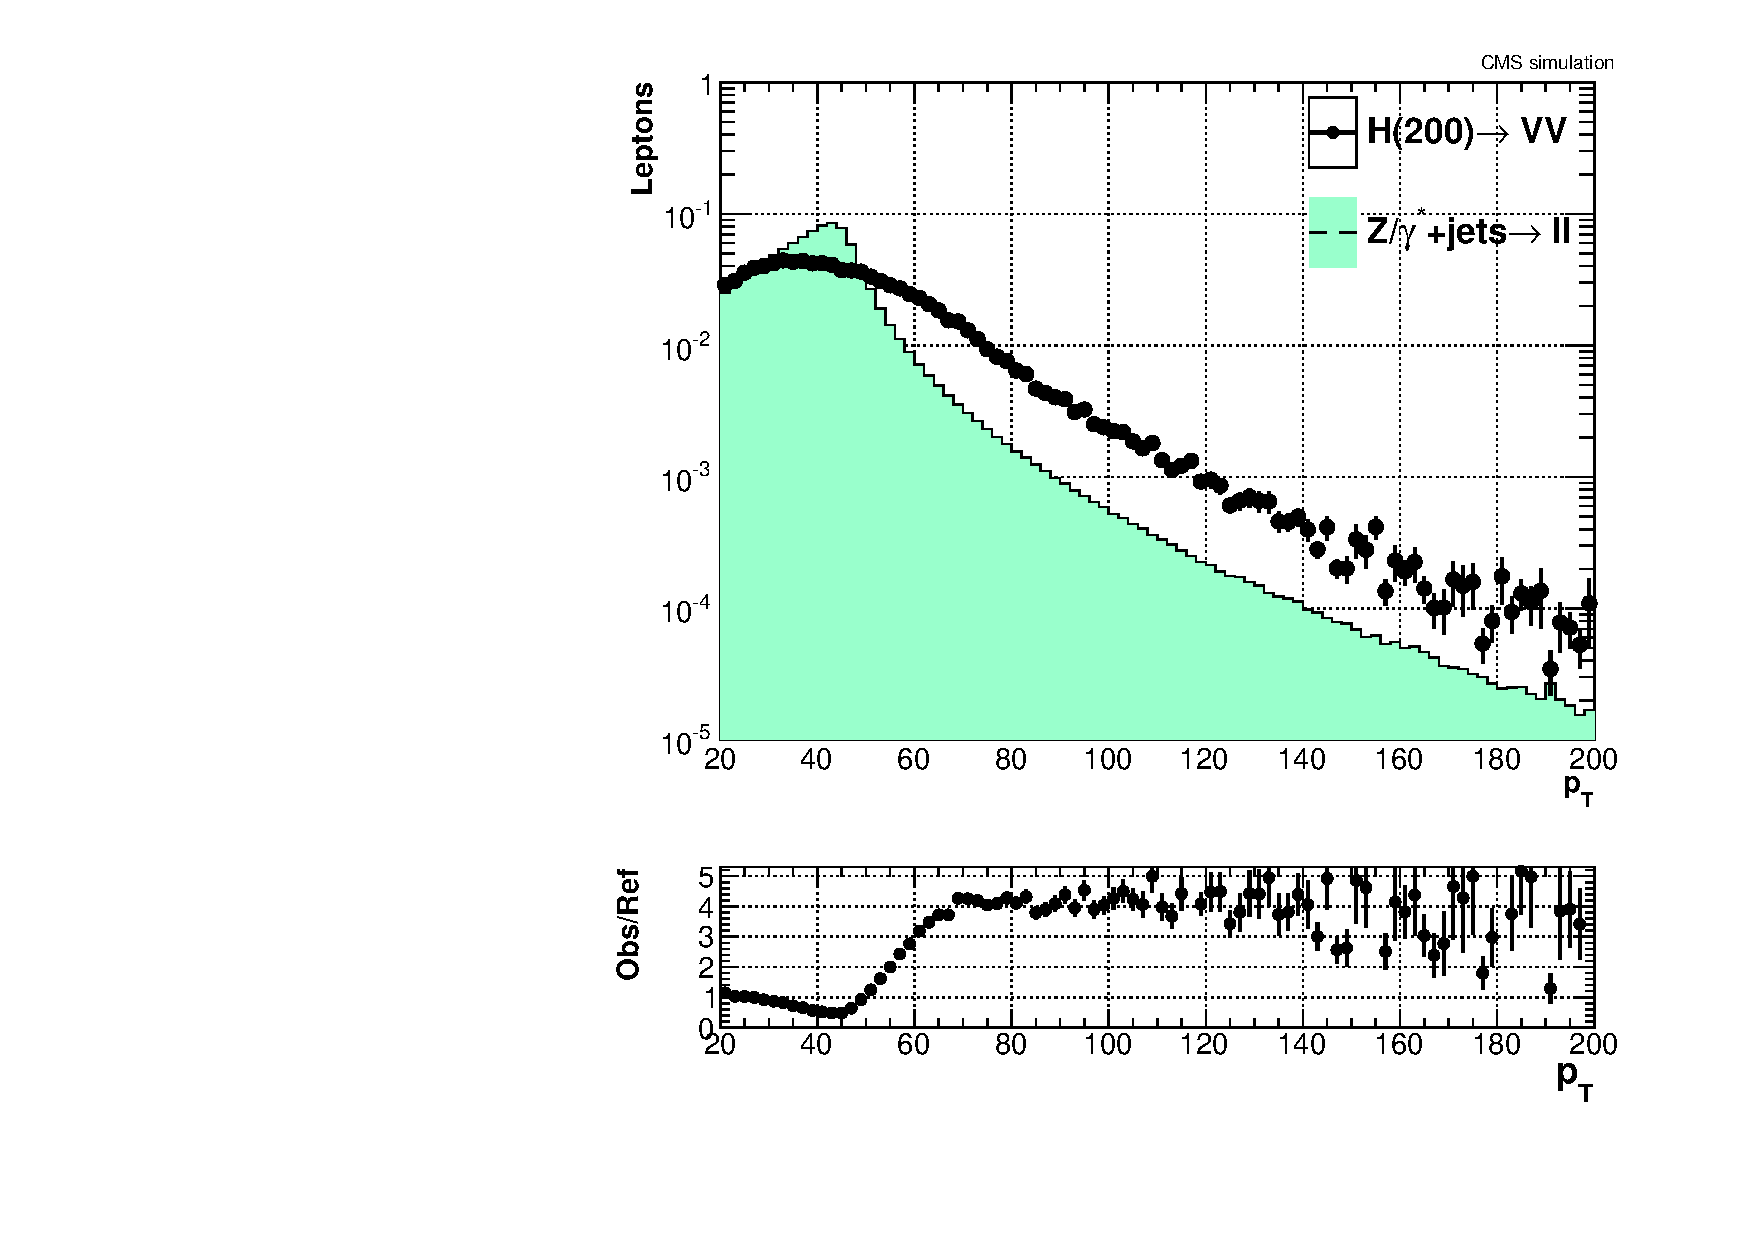
\includegraphics[width=0.3\textwidth]{img/matchedmuon_pt}
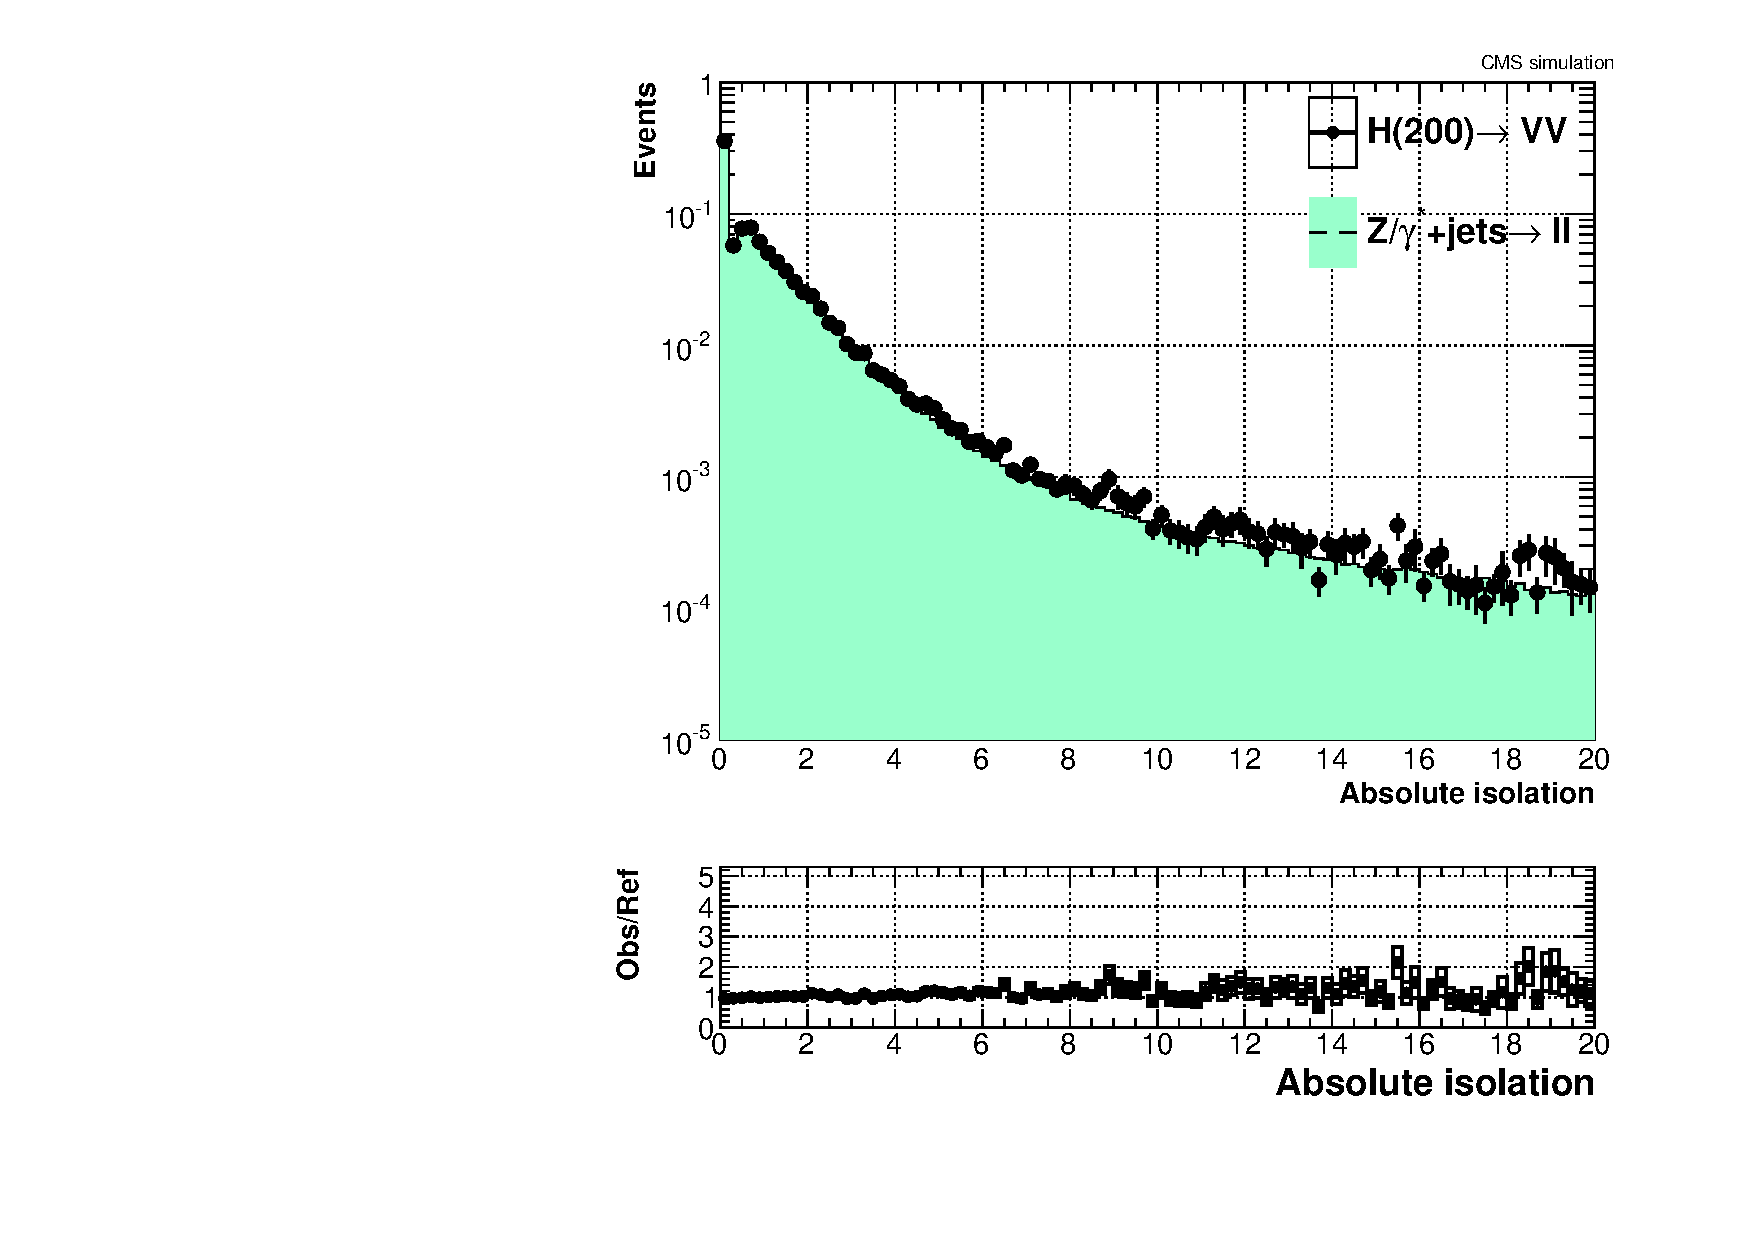
\includegraphics[width=0.3\textwidth]{img/matchedmuon_absiso}
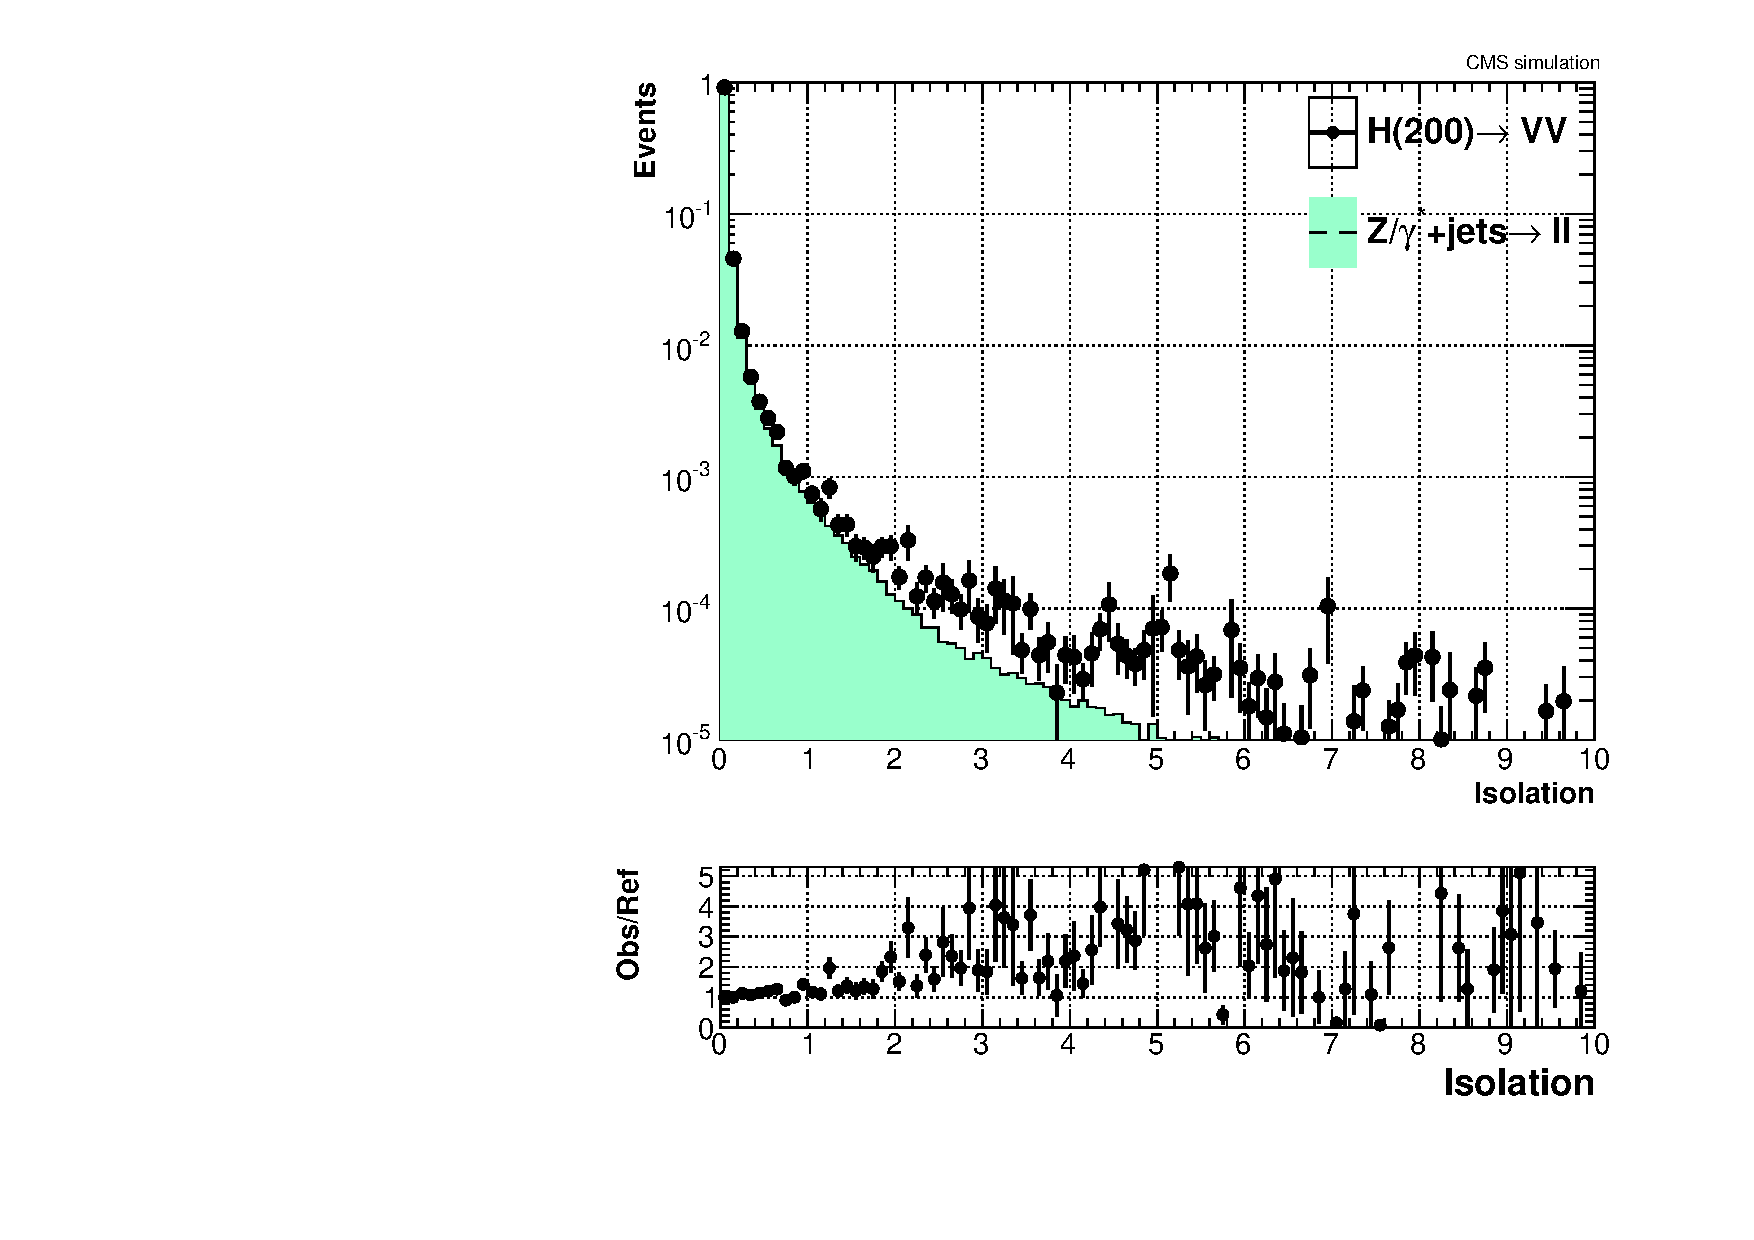
\includegraphics[width=0.3\textwidth]{img/matchedmuon_reliso}\\
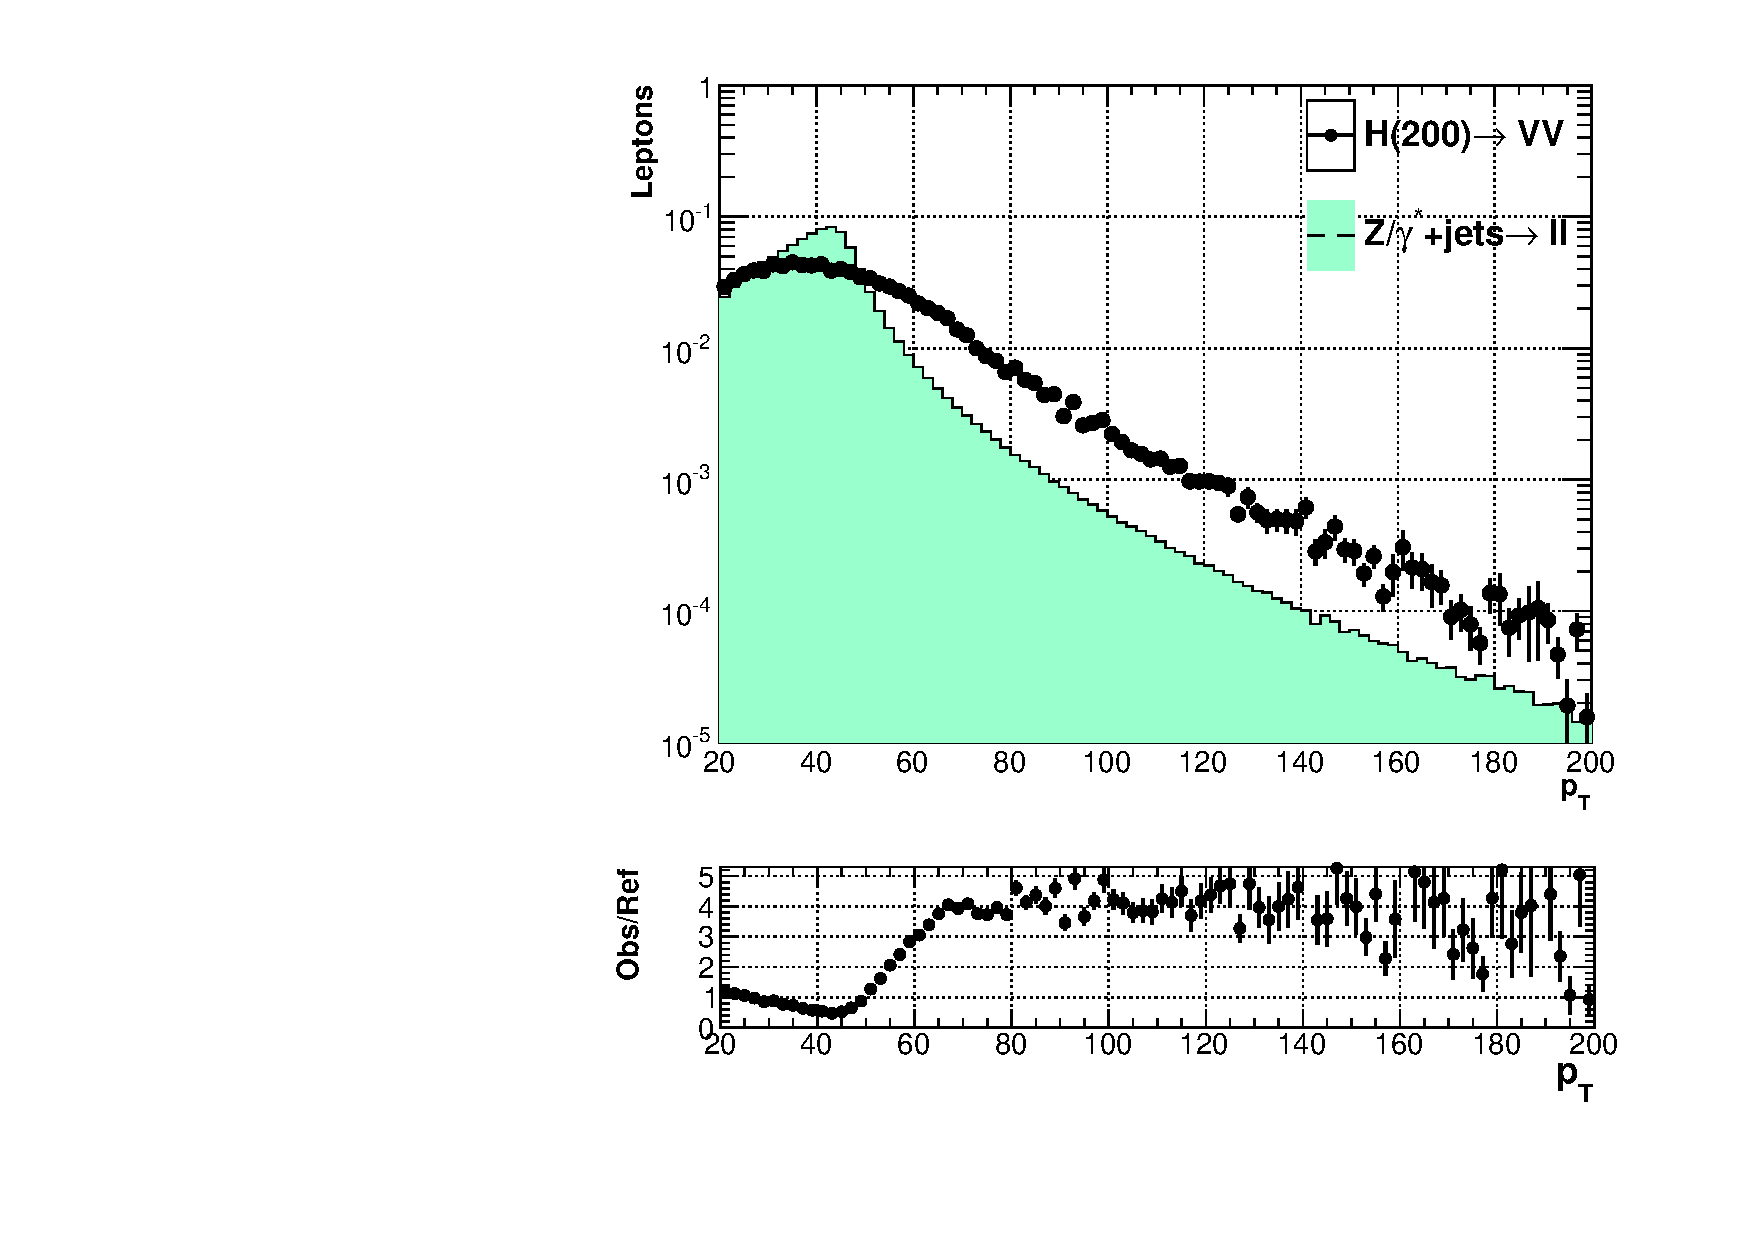
\includegraphics[width=0.3\textwidth]{img/matchedelectron_pt}
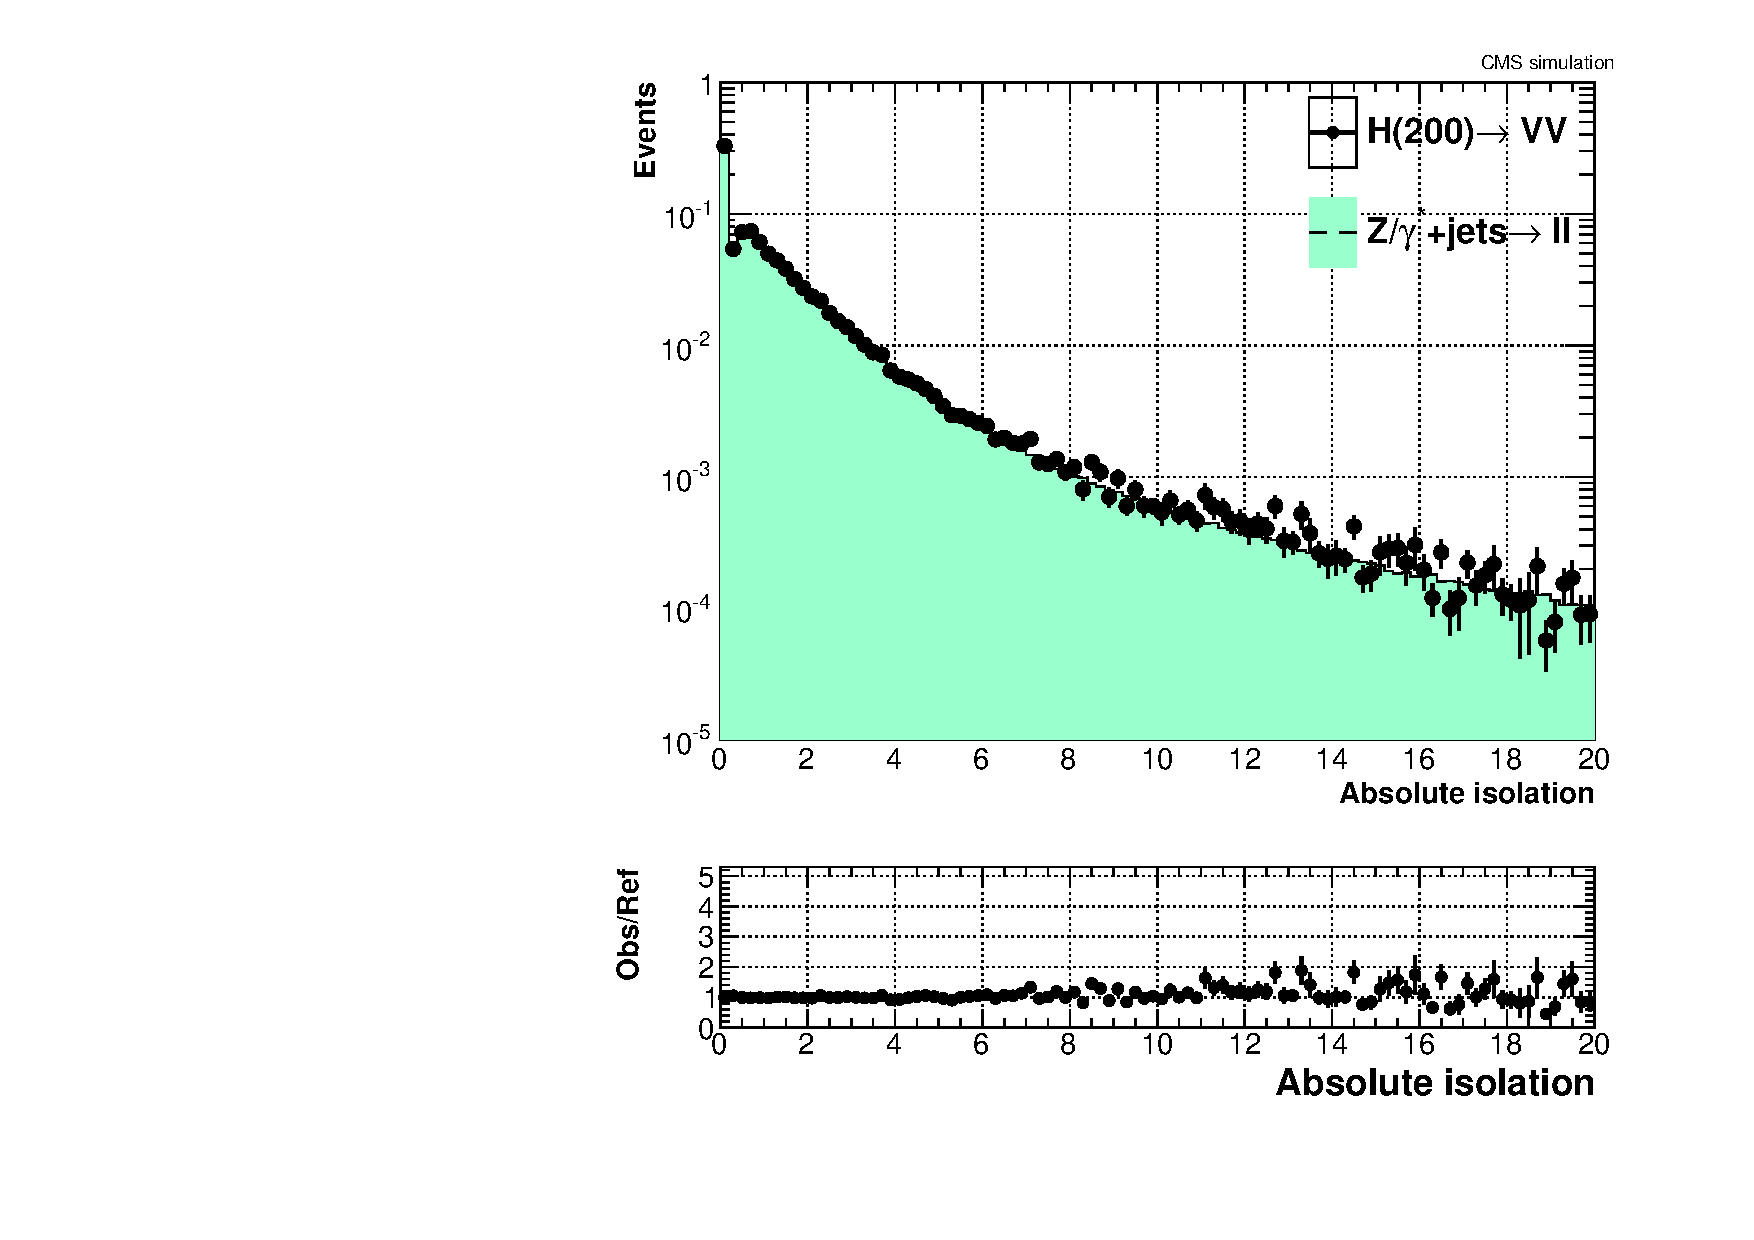
\includegraphics[width=0.3\textwidth]{img/matchedelectron_absiso}
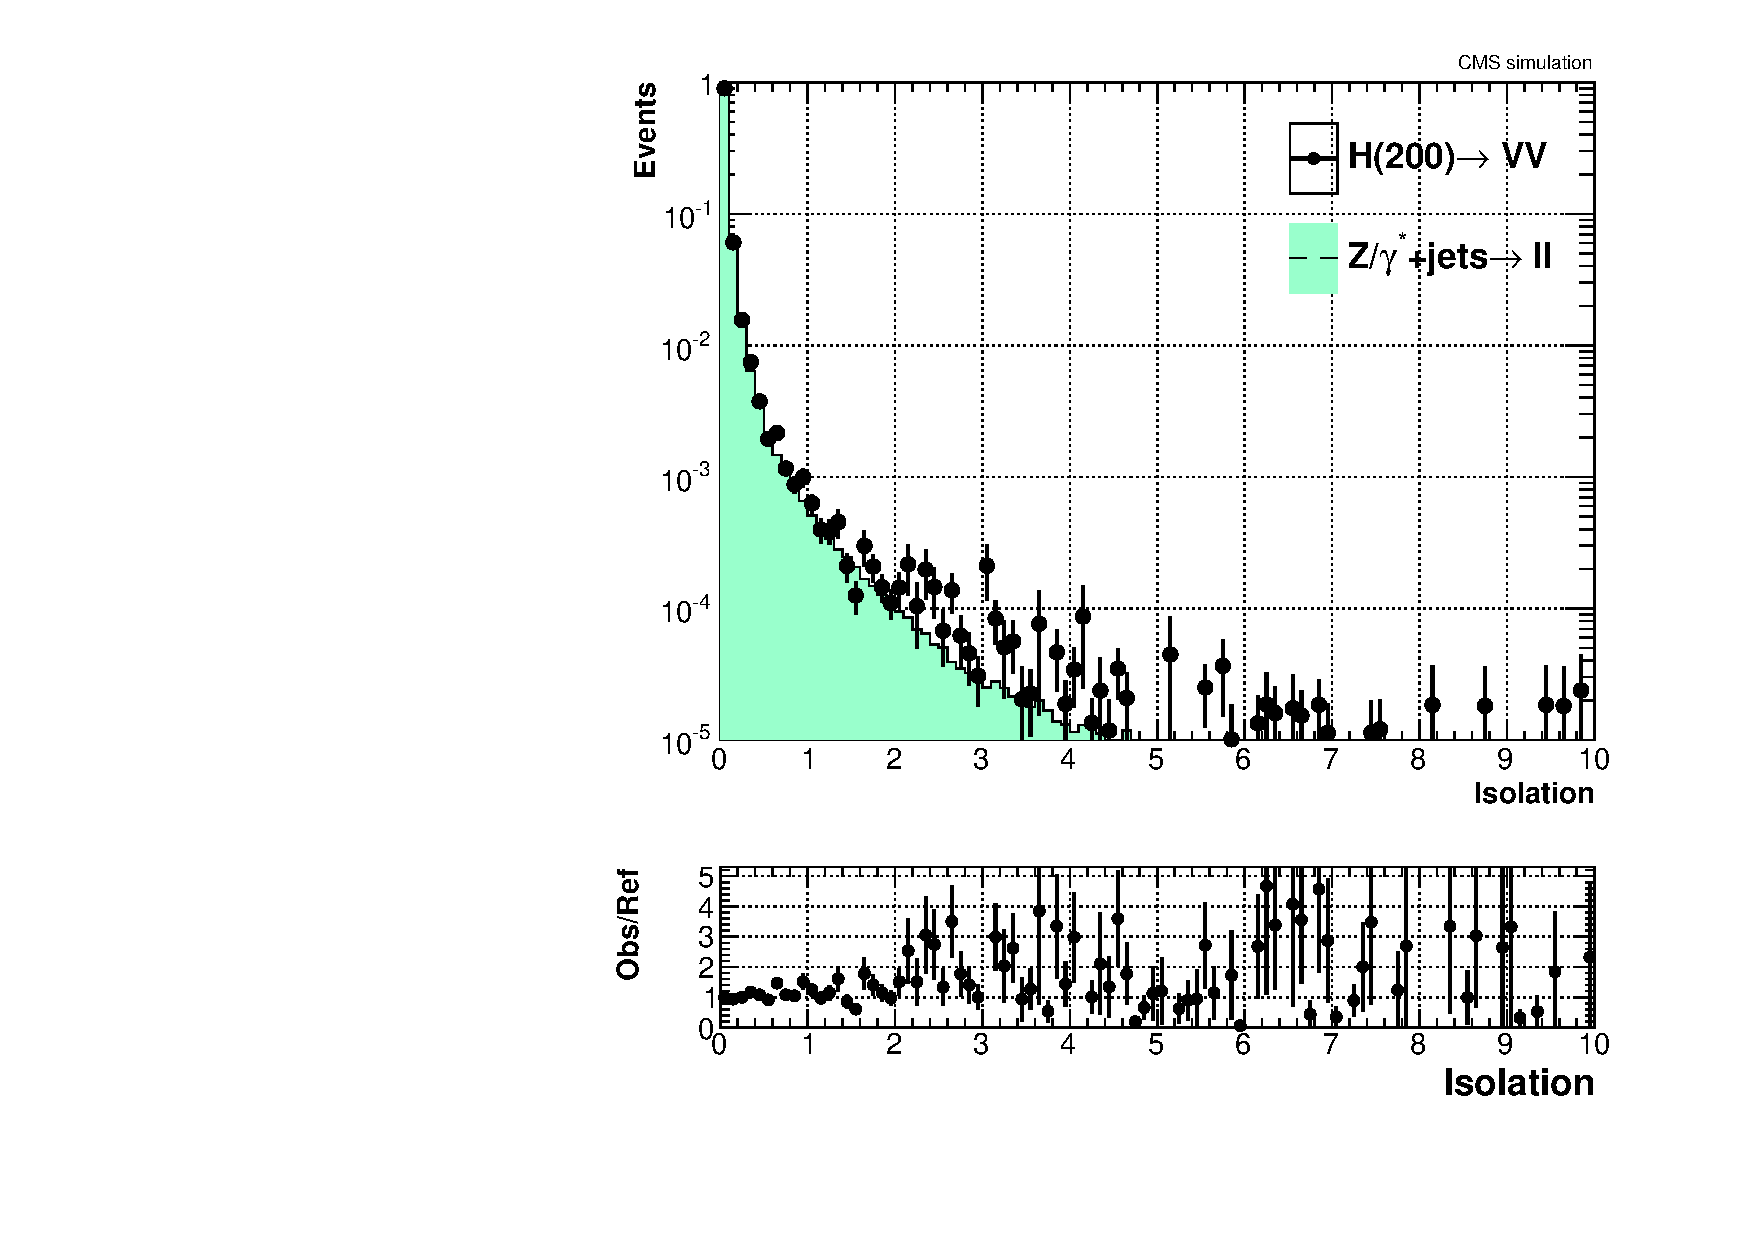
\includegraphics[width=0.3\textwidth]{img/matchedelectron_reliso}
\caption{Transverse momentum ({\em left}), absolute isolation ({\em center}) and relative isolation ({\em right}) of the
reconstructed muons ({\em top}) and electrons ({\em bottom}) matched to the generator level
leptons fro the $Z$ boson decay in simulation.
The standard $Z$ production is compared to the production in the Higgs decay chain considering an hypothetical mass of 200~GeV/c$^2$.}
\label{fig:zvshlepkinematics}
\end{center}
\end{figure}




  
\end{document}


